\chapter{Некоторые физические свойства трёхкомпонентных халькогенидов меди} \label{chapt4}
В данной главе представлены результаты экспериментальных исследований зависимостей намагниченности в диапазоне температур от 2 до 350~К и спектров комбинационного рассеяния света для соединений Cu\textsubscript{12}As\textsubscript{4}S\textsubscript{13}, Cu\textsubscript{12}Sb\textsubscript{4}S\textsubscript{13}, Cu\textsubscript{3}AsSe\textsubscript{3} и Cu\textsubscript{3}SbSe\textsubscript{3} при комнатной температуре. А также измерение теплоёмкости в диапазоне температур от 4 до 350~К и результаты моделирования теплоёмкости для Cu\textsubscript{12}As\textsubscript{4}S\textsubscript{13} и Cu\textsubscript{3}AsSe\textsubscript{3}.

\section{Температурные зависимости магнитной восприимчивости трёхкомпонентных халькогенидов меди} \label{sect4_1}

Полученные графики зависимости магнитной восприимчивости (рис. \ref{img:magsus1} и \ref{img:magsus2}) обладают видом, характерным для парамагнетиков с областями отклонения от парамагнитного хода.  Температурные зависимости магнитной восприимчивости для каждого образца были получены в магнитных полях 1, 10, 35 и 70~кЭ. При любом значении магнитного поля графики зависимости магнитной восприимчивости от температры обладают теми же характерными особенностями для каждого образца. Для части образцов были измерены петли гистерезиса, которые показали незначительное наличие ферромагнитных примесей. Также зависимости магнитной восприимчивости для монокристаллического и поликристаллического образцов соединения Cu\textsubscript{12}As\textsubscript{4}Se\textsubscript{13} не отличаются. Все зависимости магнитной восприимчивости приведены с вычетом диамагнитного вклада.

График зависимости для монокристаллического образца Cu\textsubscript{12}As\textsubscript{4}Se\textsubscript{13} в диапазоне температур от 2 до 200 К имеет вид отличный от кривой Кюри"--~Вейса.
 Характер кривой, измеренной магнитной восприимчивости образца  Cu\textsubscript{12}As\textsubscript{4}S\textsubscript{13}, показывает наличие возможного перехода из парамагнитного состояния в антиферромагнитное в диапазоне температур от 120 до 130~К (\ref{img:magsus1}а).
До температуры 170 К зависимость парамагнитного вклада магнитной восприимчивости монотонно возрастает с понижением температуры и согласуется с Кюри"--~Вейсовским поведением, характерным для парамагнетика.

\begin{figure}[p!]
  \begin{minipage}[ht]{0.9\linewidth}\centering
    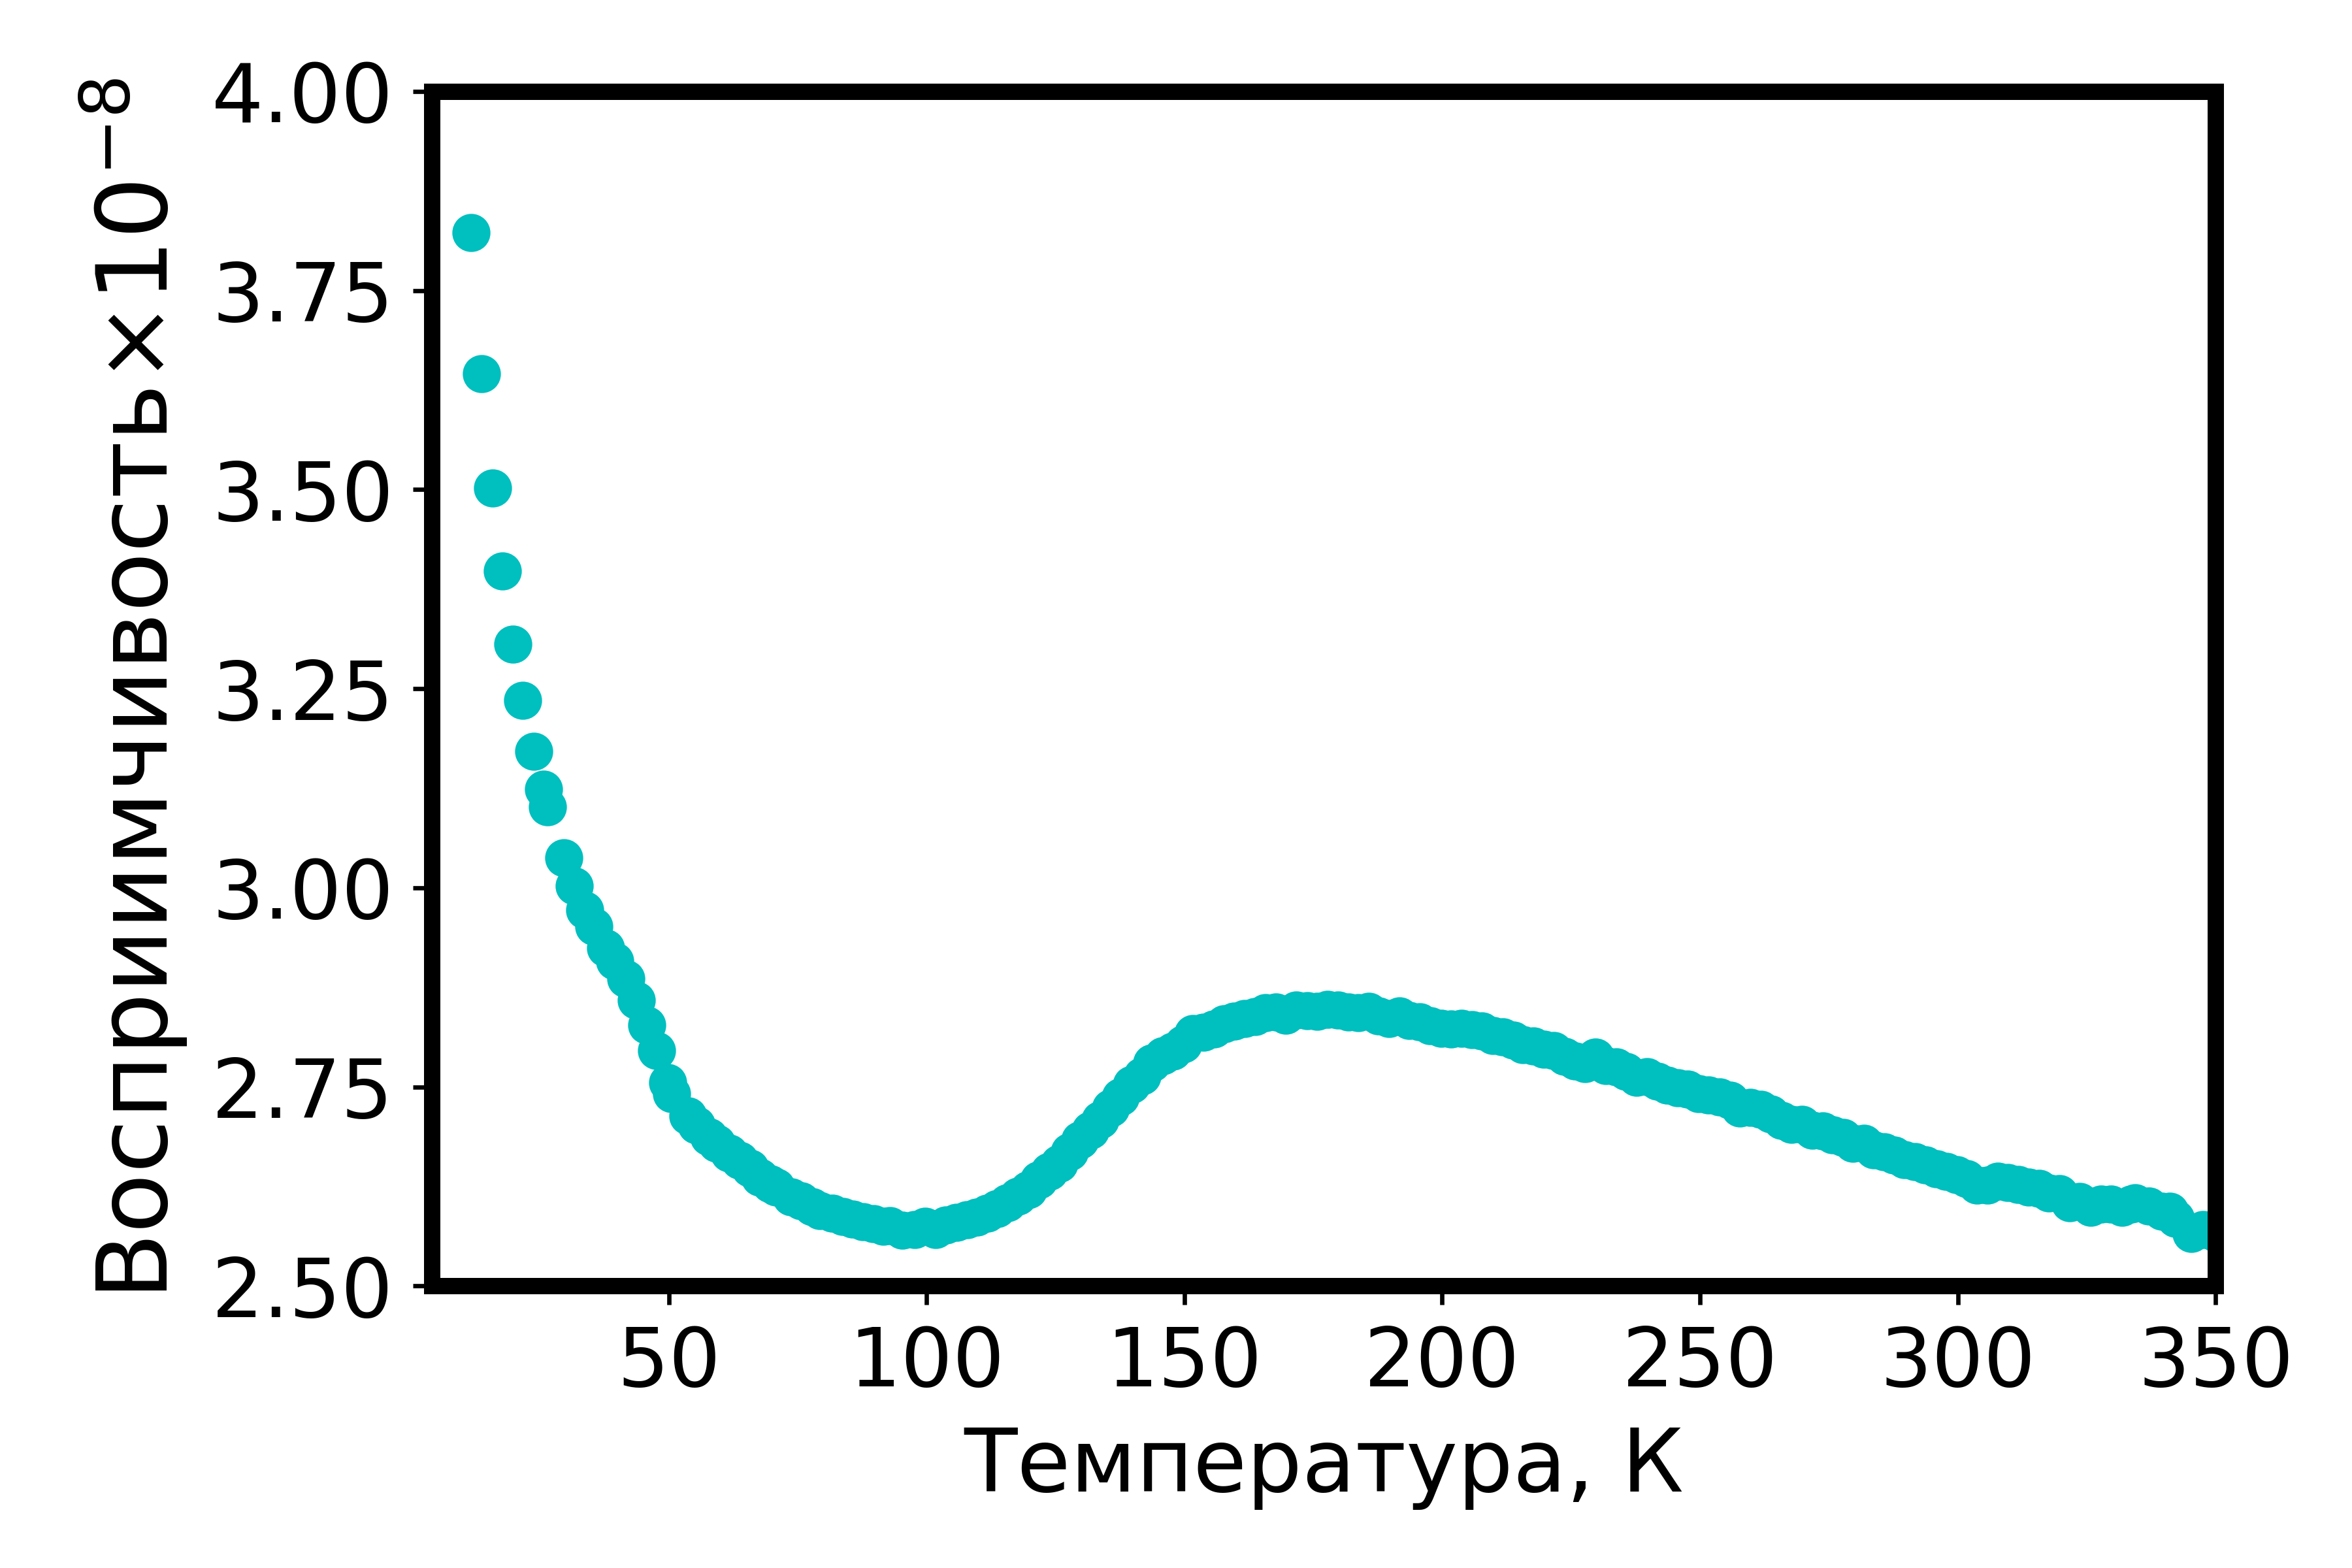
\includegraphics[width=0.9\linewidth]{sus_exp_Cu_As_S} \\ а)
  \end{minipage}
 \vfill
  \begin{minipage}[ht]{0.9\linewidth}\centering
    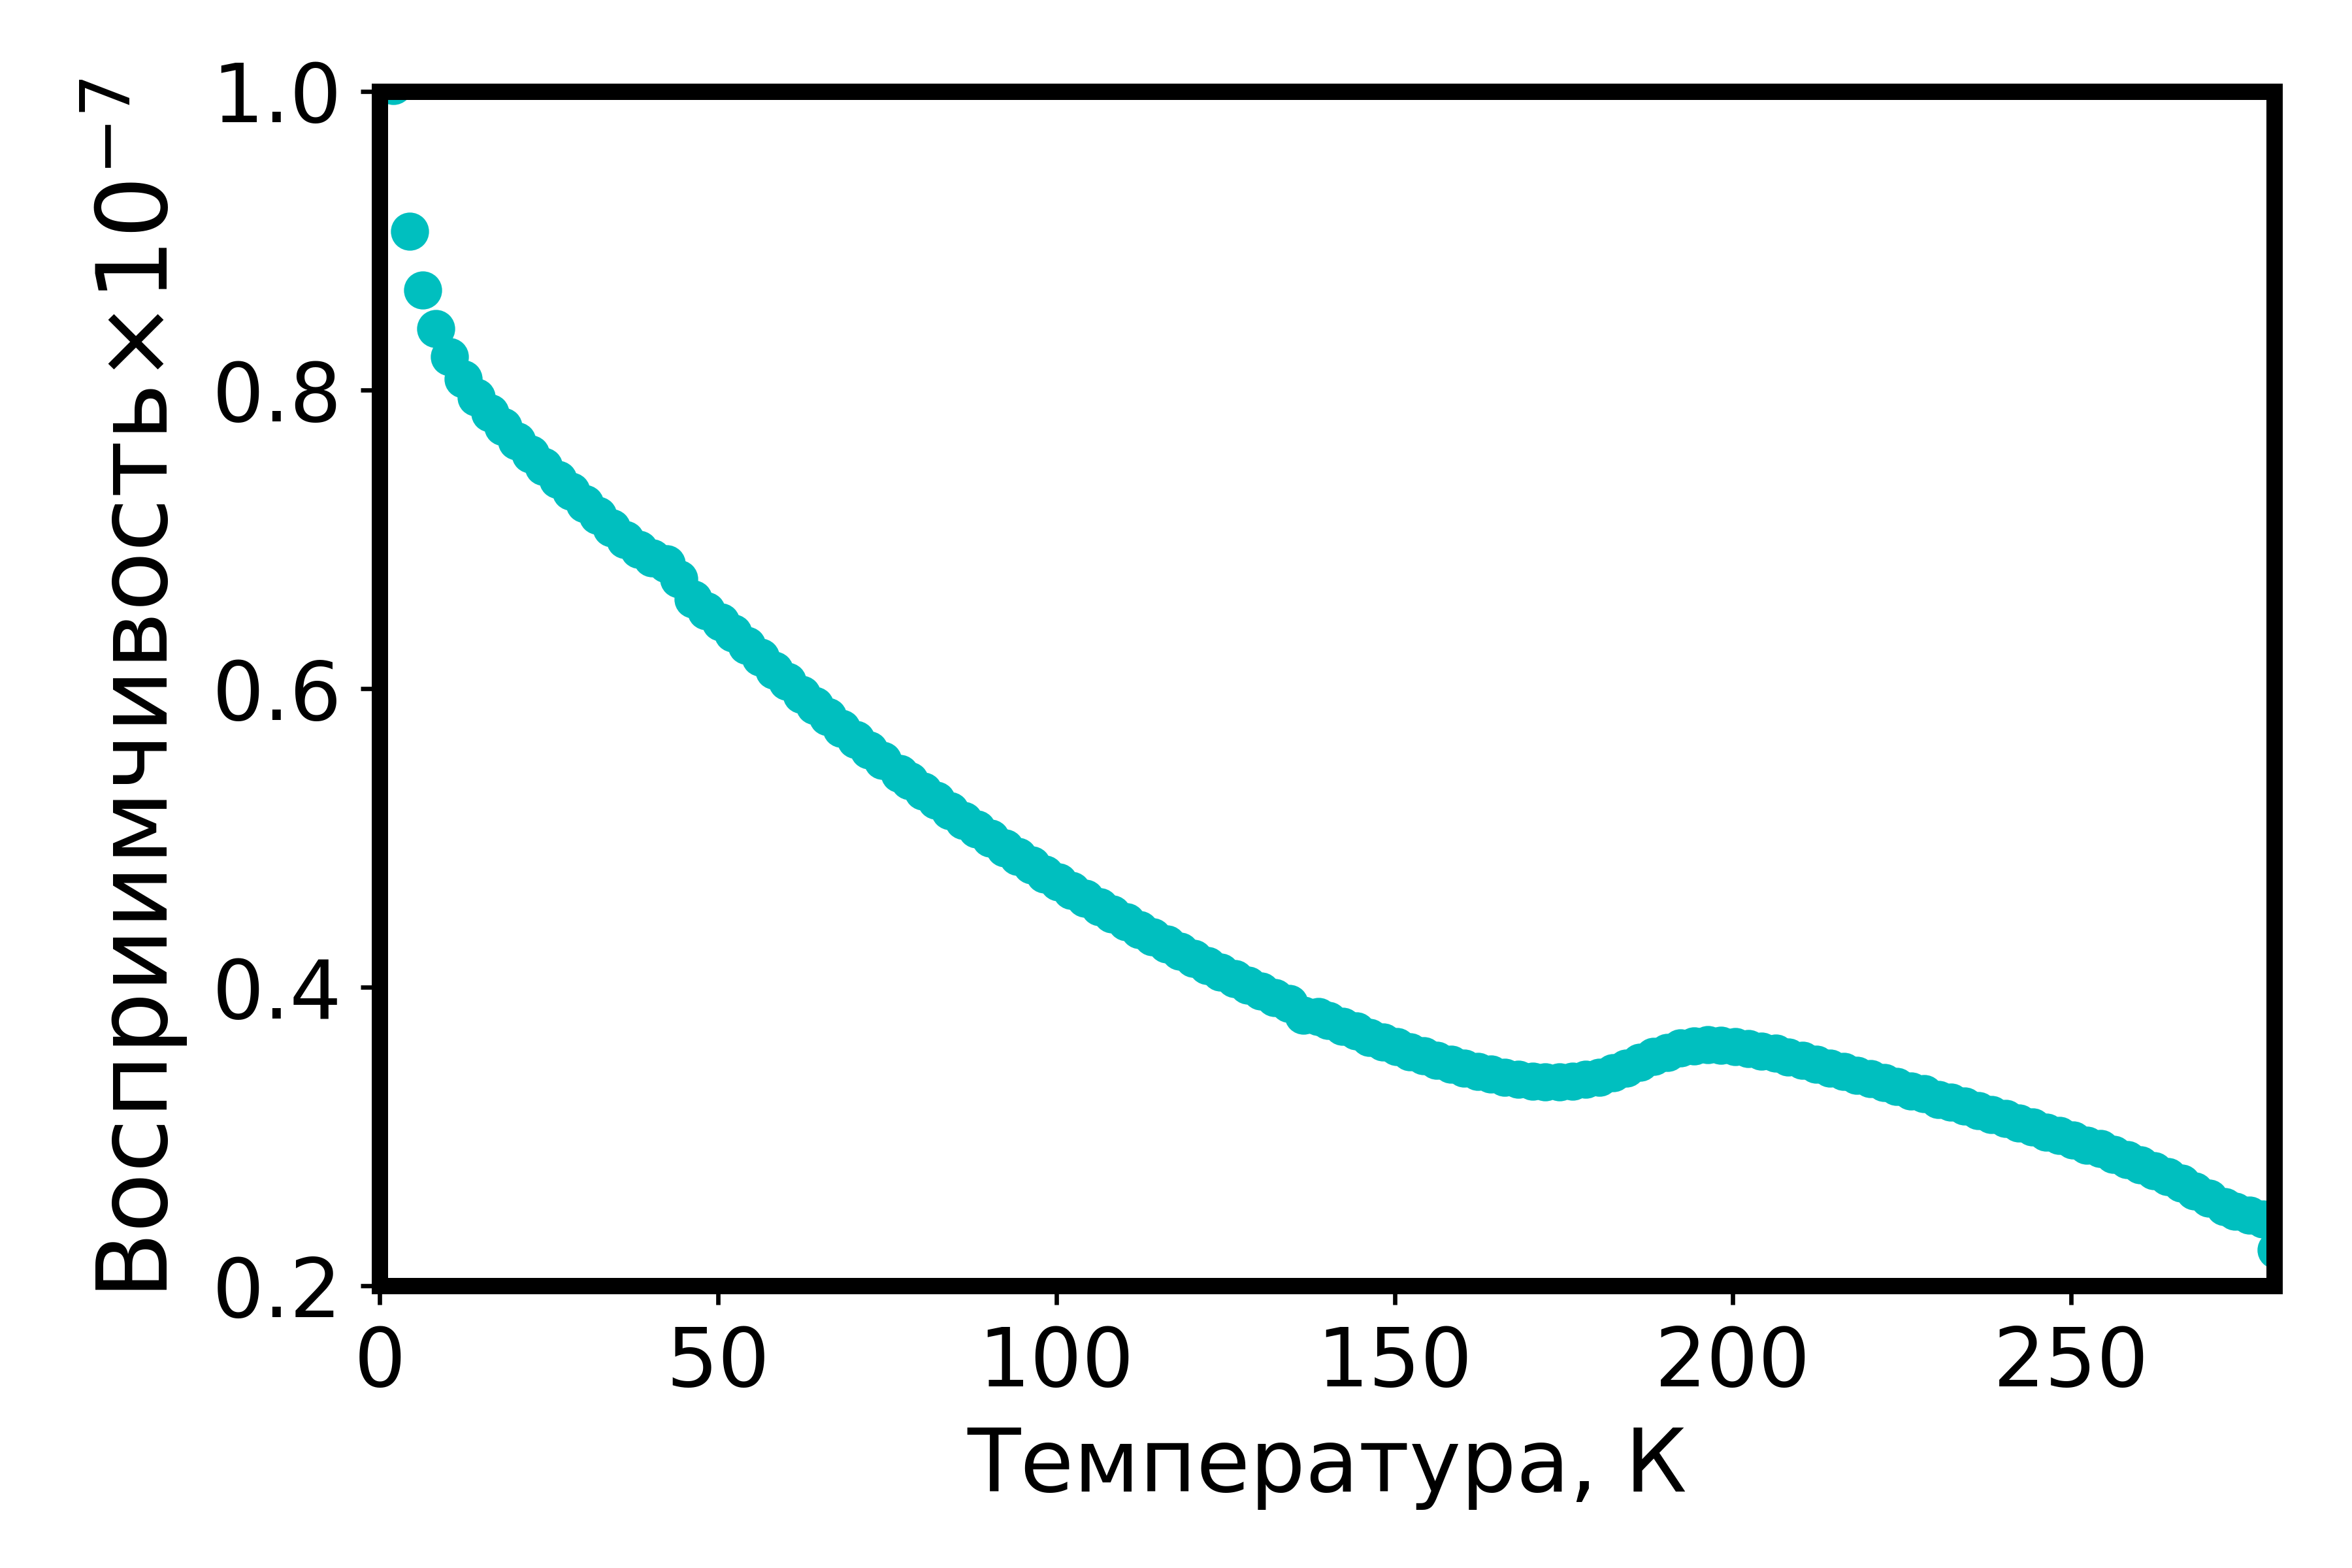
\includegraphics[width=0.9\linewidth]{sus_exp_Cu_As_Se} \\ б)
  \end{minipage}
      \caption[Графики зависимости магнитной восприимчивости для образцов Cu\textsubscript{12}As\textsubscript{4}Se\textsubscript{13} (а) и Cu\textsubscript{3}AsS\textsubscript{3} (б)]{Графики зависимости магнитной восприимчивости для образцов Cu\textsubscript{12}As\textsubscript{4}S\textsubscript{13} (а) и Cu\textsubscript{3}AsSe\textsubscript{3} (б)}
    \label{img:magsus1}
\end{figure}

График зависимости удельной намагниченности образца Cu\textsubscript{3}AsSe\textsubscript{3} от температуры, измеренный в магнитном поле напряженностью 10 кЭ, представлен на рис. \ref{img:magsus1}б.
При температуре 44 К наблюдается пик магнитной восприимчивости, в интервале температур 170--200 К происходит рост магнитной восприимчивости, а при температуре 285--295 К её падение.
По-видимому, в интервале температур 170--295 К реализуется особое магнитное состояние в соединении синтетического мгриита.

При температурах 2, 250 и 300~К измерены петли гистерезиса (рис. \ref{img:magsus3}) для образца Cu\textsubscript{3}AsSe\textsubscript{3}.
Рост намагниченности при увеличении температуры при 2 и 250 К также говорит о
том, что исследуемое соединение является парамагнетиком.
Однако, для температур выше 300 К намагниченность становится отрицательной, что
говорит о доминировании диамагнетизма.
 Ветви петли гистерезиса располагаются во втором и четвертом квадрантах, что соответствует диамагнетикам.
Детальное исследование в области малых магнитных полей при учете парамагнетизма (при 2 и 250 К) или диамагнетизма (при 300 К) позволили обнаружить слабый ферромагнетизм в исследуемом соединении, который, по-видимому, связан с наличием ферромагнитных примесей в синтезированном соединении.
Увеличенные петли гистерезиса представлены на вставке рисунка \ref{img:magsus3}.



\begin{figure}[pt!]
  \begin{minipage}[ht]{0.9\linewidth}\centering
    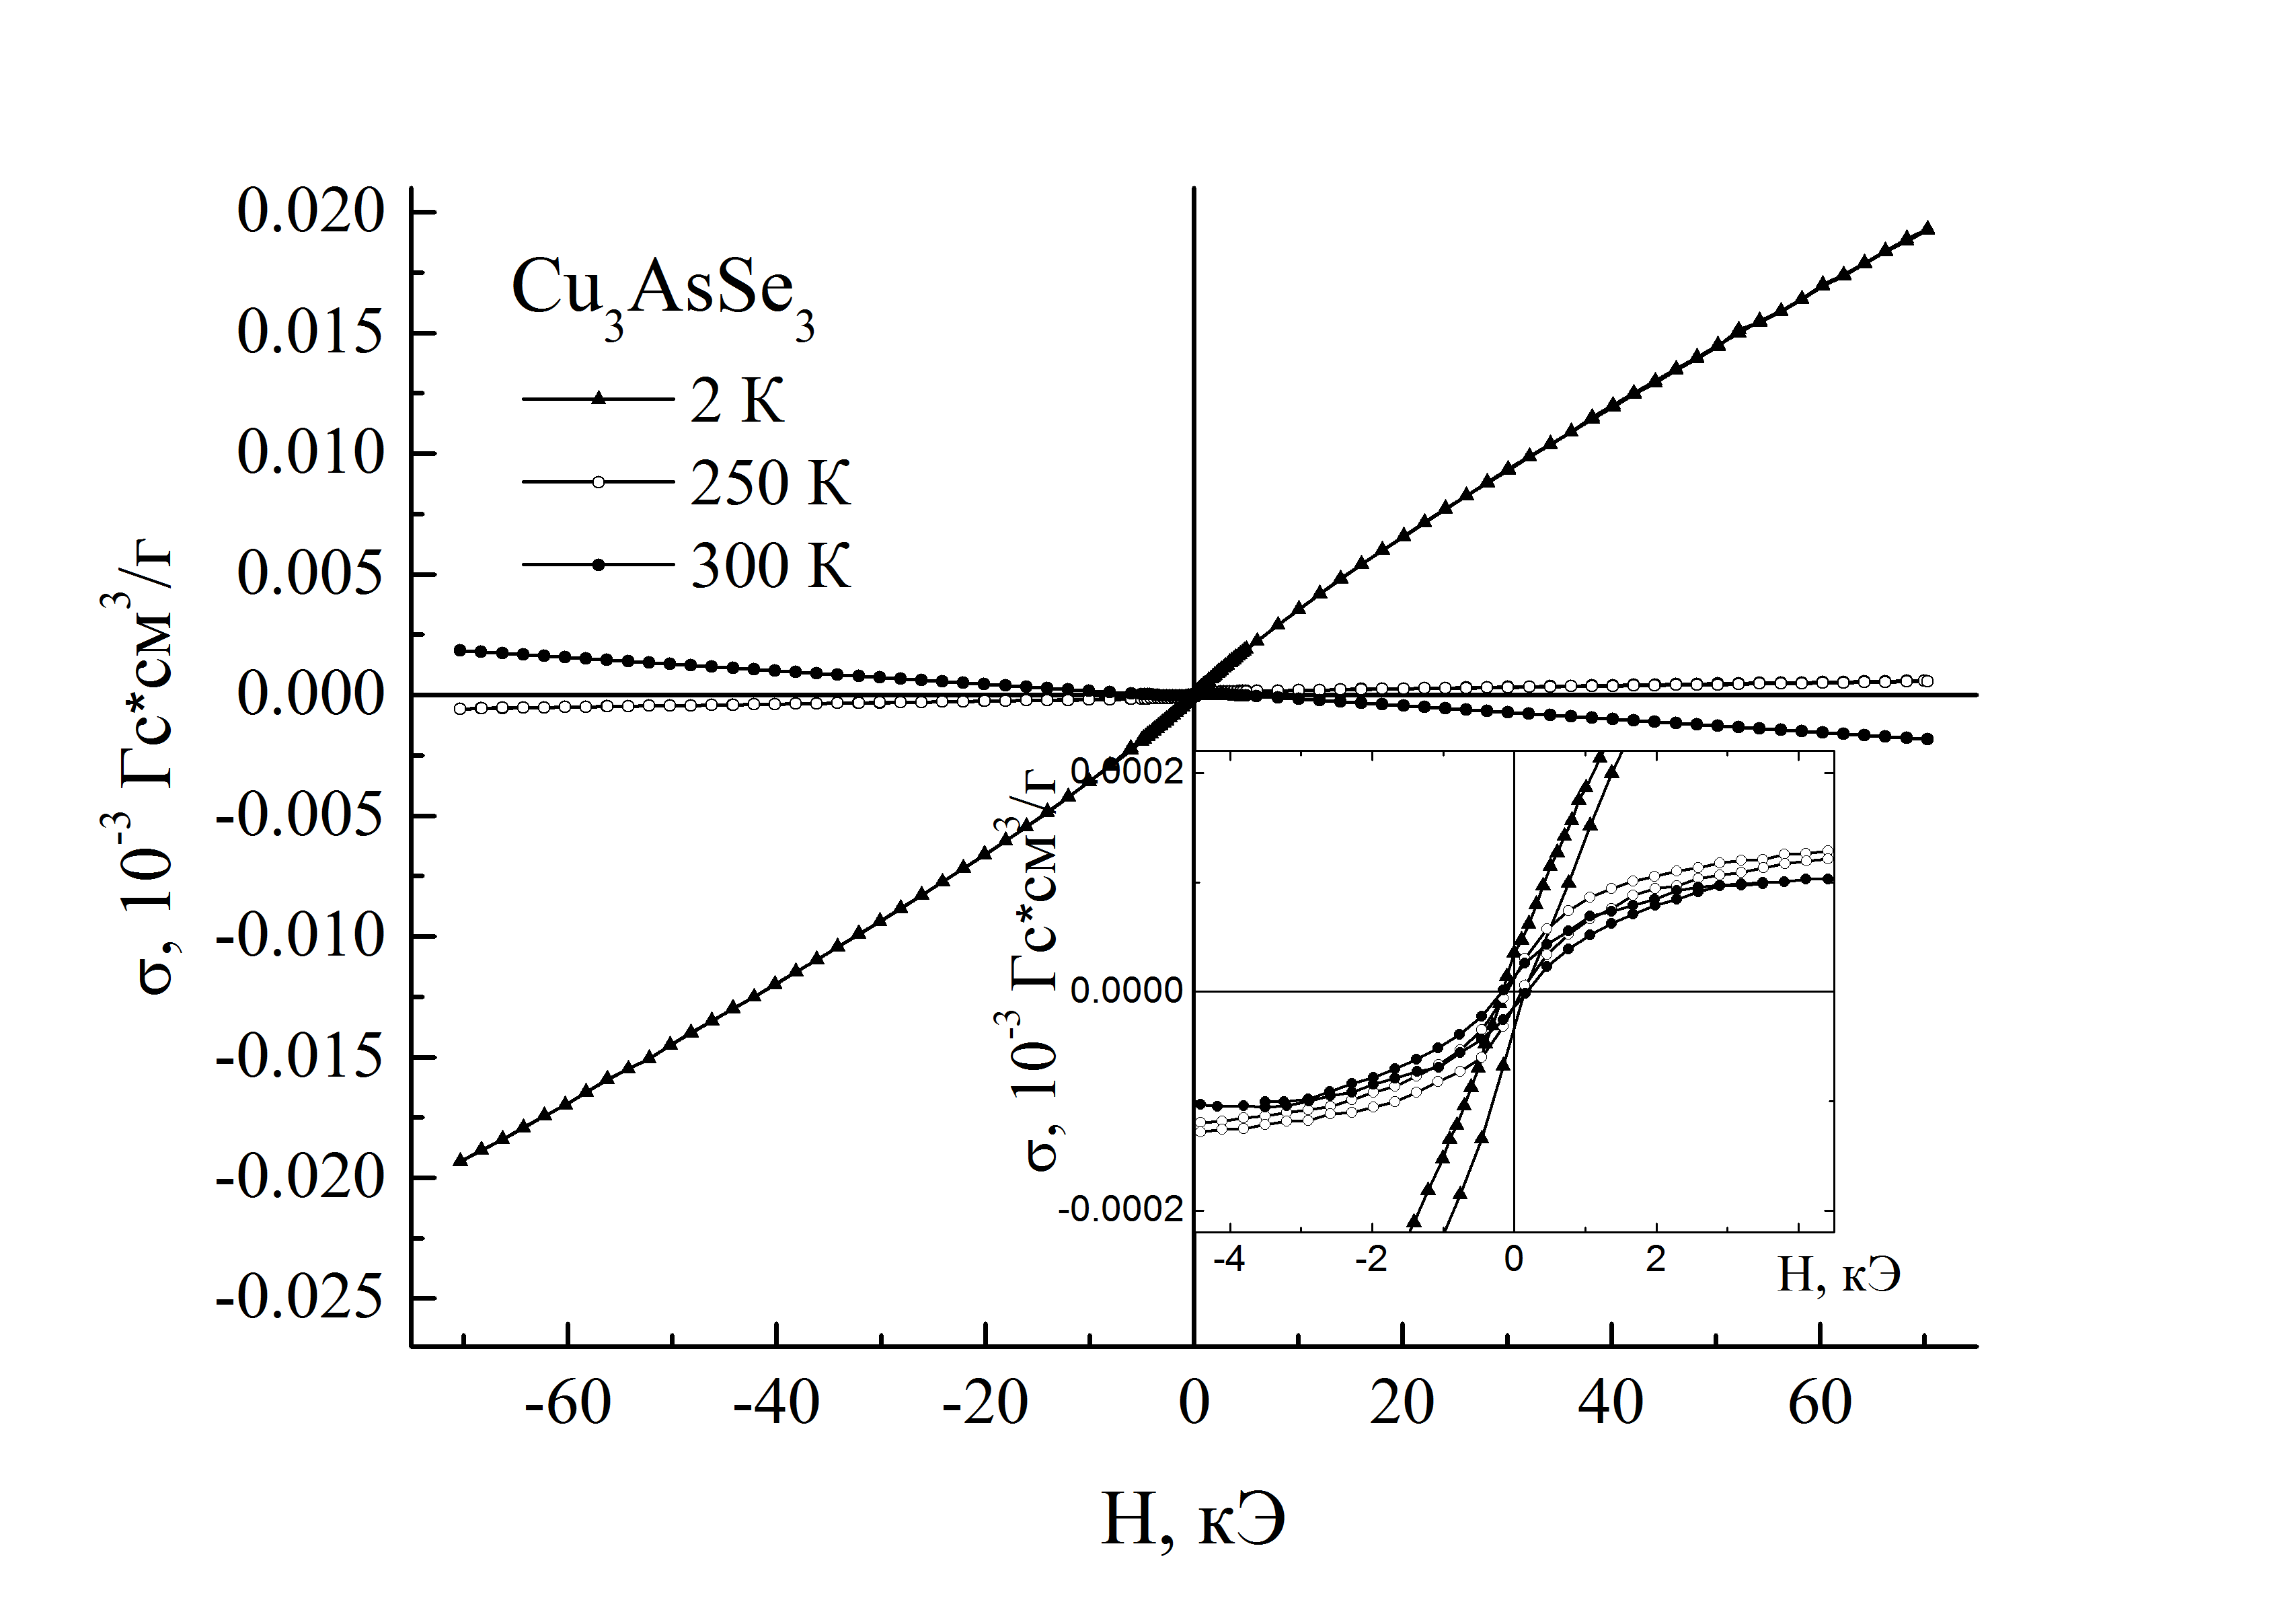
\includegraphics[width=0.9\linewidth]{sigma_mag} \\
  \end{minipage}

      \caption[Графики зависимости удельной намагниченности в магнитных полях от $-$70 до 70~кЭ при температурах 2, 250 и 300~К для образца Cu\textsubscript{3}AsSe\textsubscript{3}]{Графики зависимости удельной намагниченности в магнитных полях от $-$70 до 70~кЭ при температурах 2, 250 и 300~К для образца Cu\textsubscript{3}AsSe\textsubscript{3}}
    \label{img:magsus3}
\end{figure}


\begin{figure}[pt!]
  \begin{minipage}[ht]{0.9\linewidth}\centering
    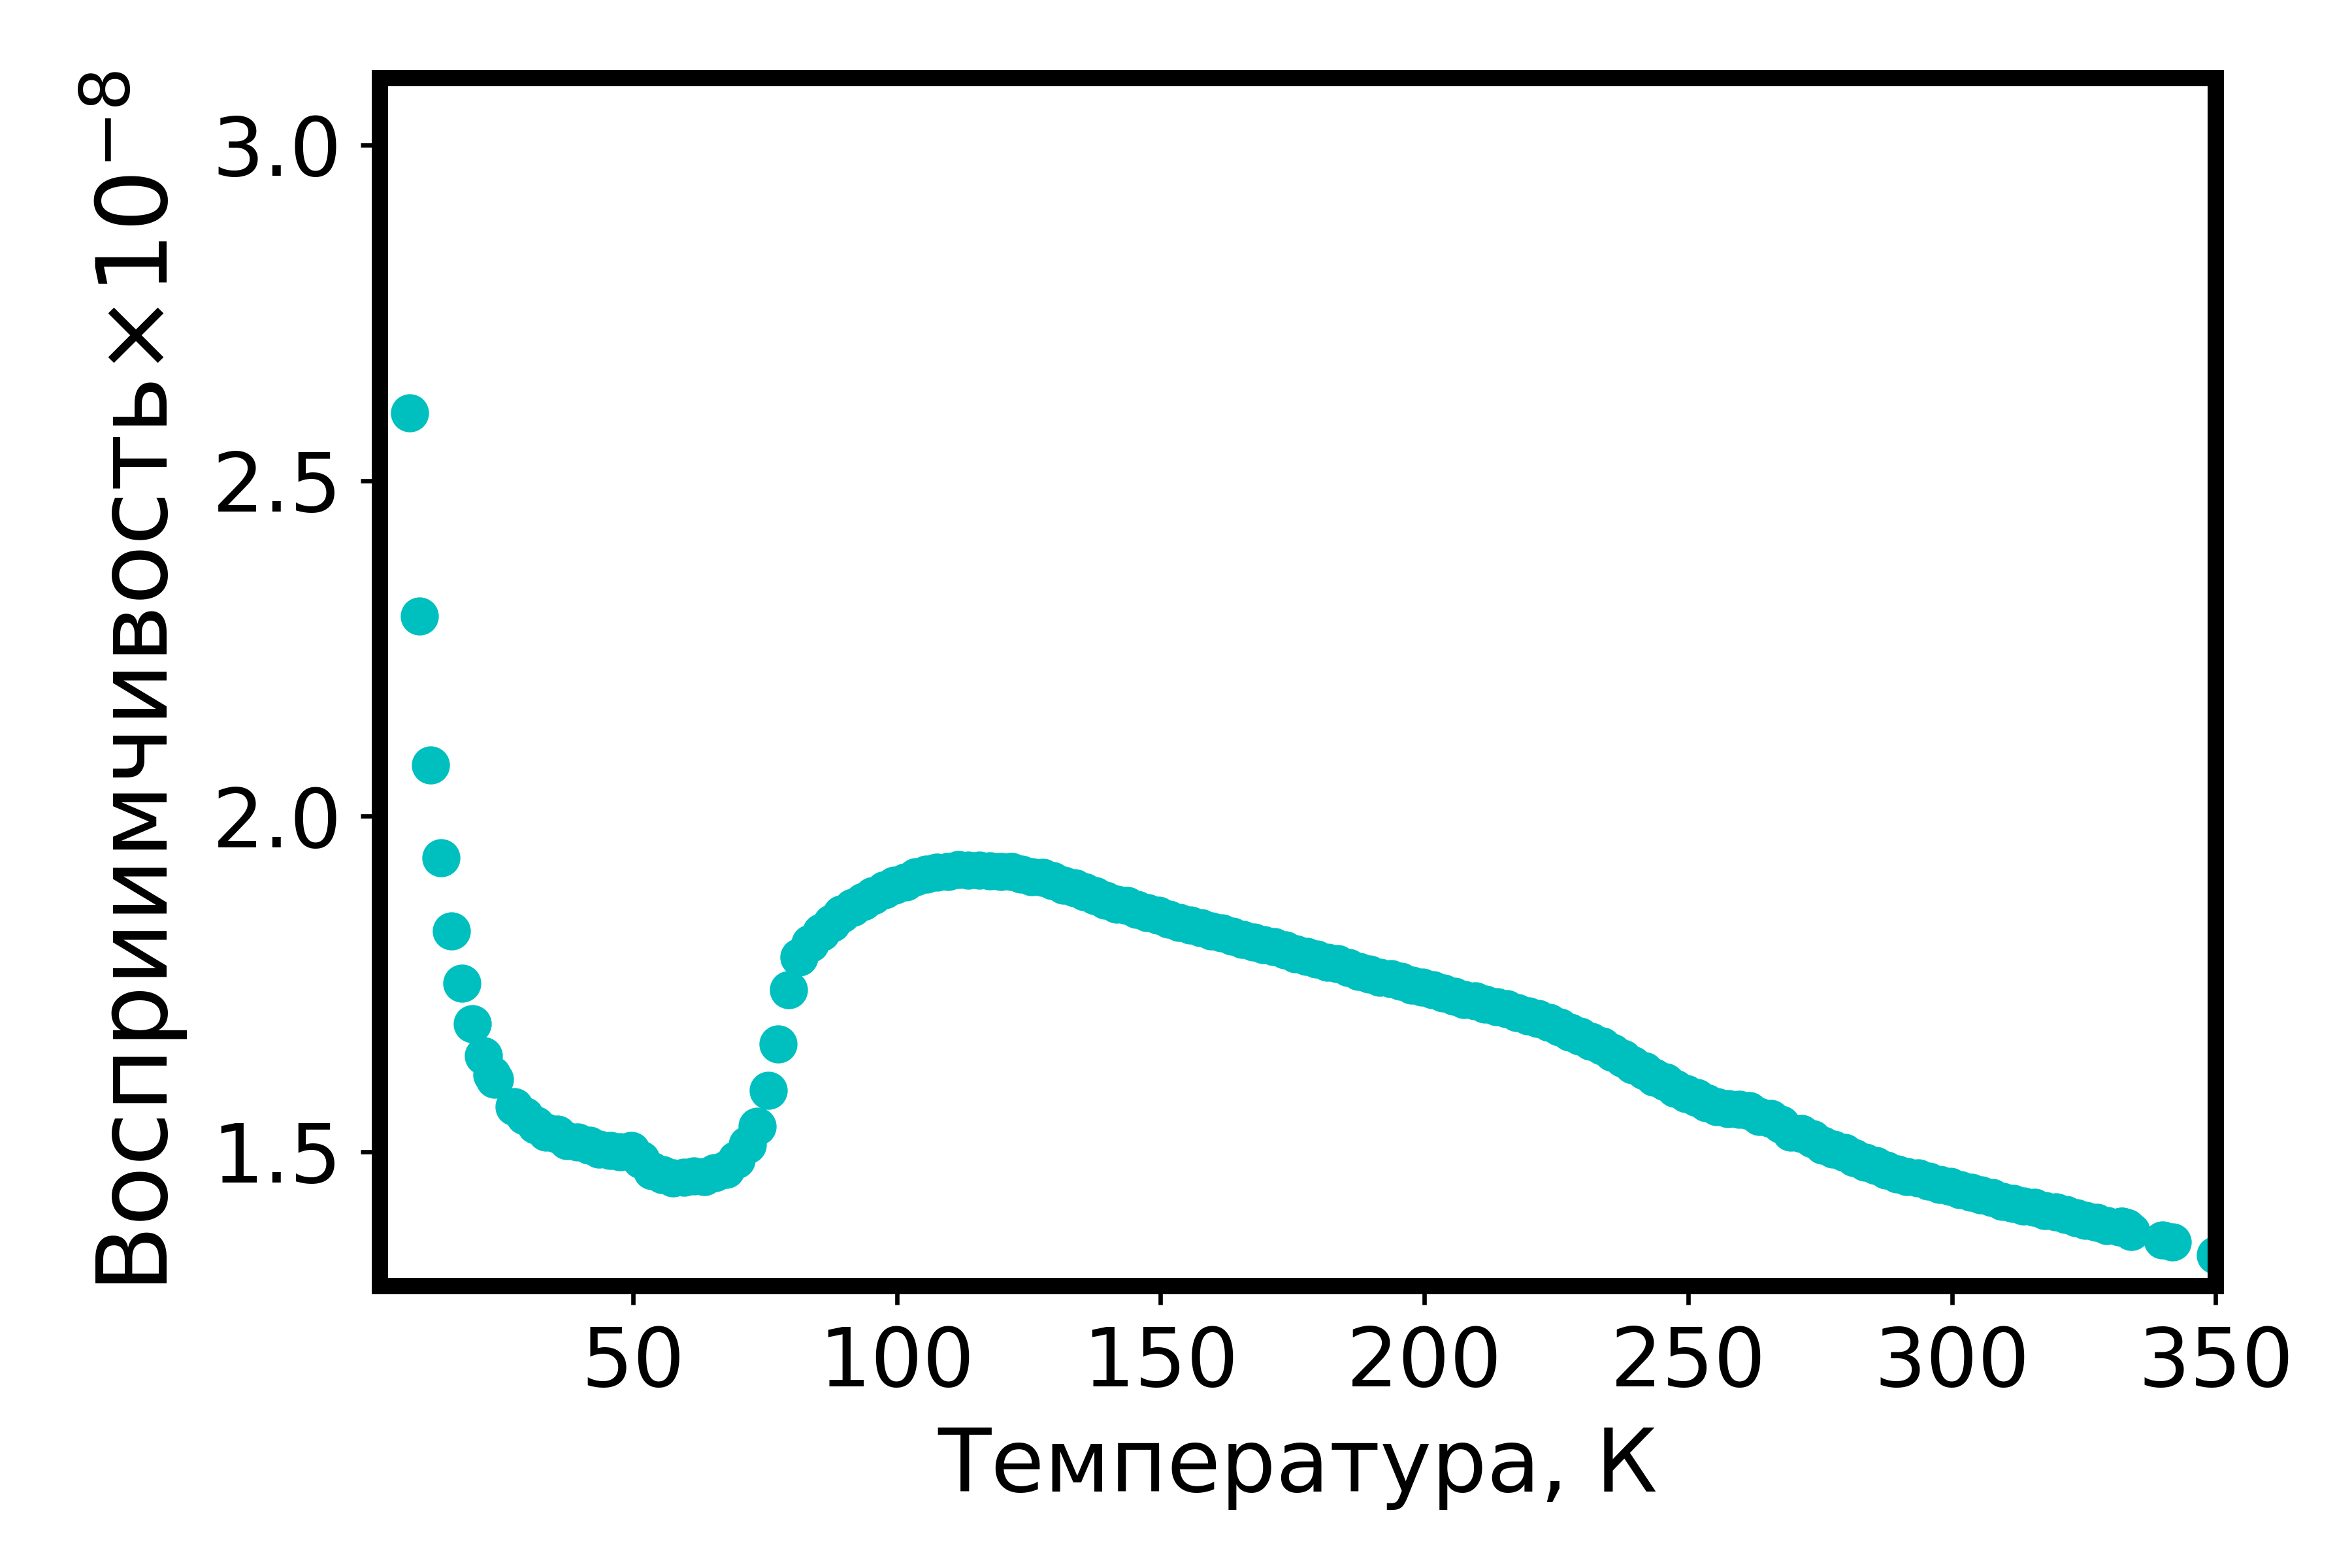
\includegraphics[width=0.9\linewidth]{sus_exp_Cu_Sb_S} \\ а)
  \end{minipage}
\vfill
  \begin{minipage}[ht]{0.9\linewidth}\centering
    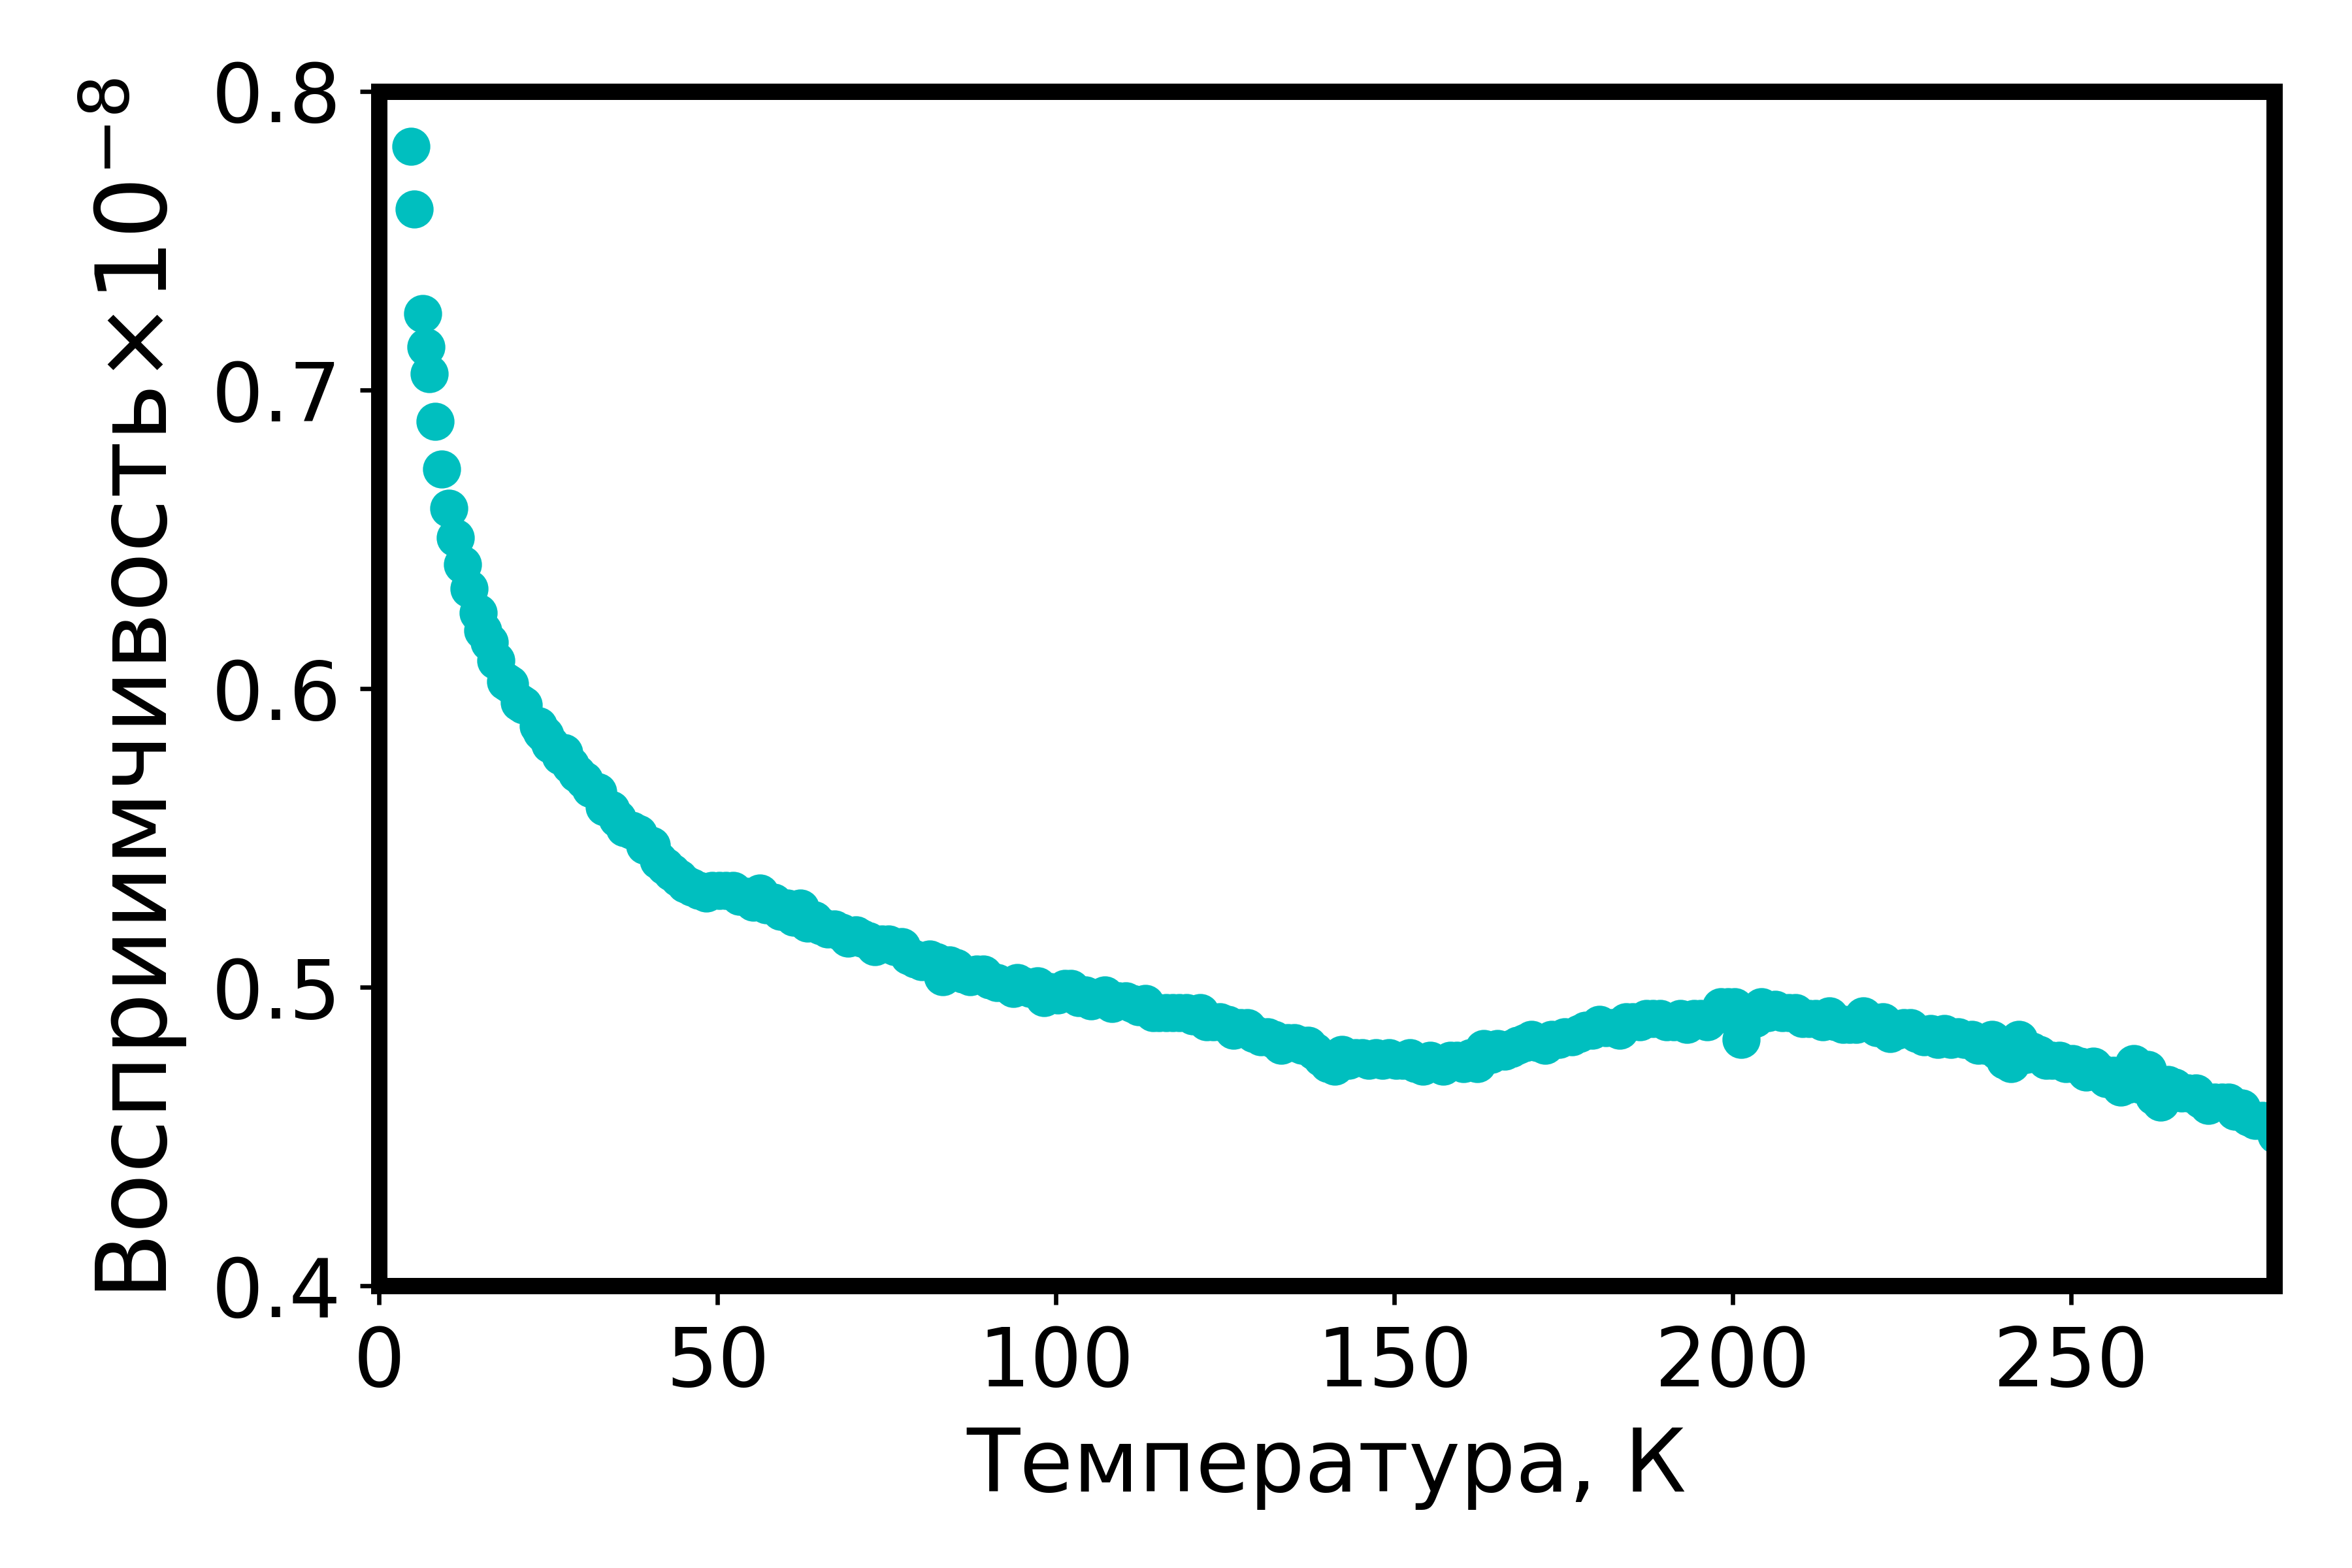
\includegraphics[width=0.9\linewidth]{sus_exp_Cu_Sb_Se} \\ б)
  \end{minipage}
      \caption[Графики зависимости магнитной восприимчивости для образцов Cu\textsubscript{12}Sb\textsubscript{4}S\textsubscript{13} (а) и Cu\textsubscript{3}SbSe\textsubscript{3} (б)]{Графики зависимости магнитной восприимчивости для образцов Cu\textsubscript{12}Sb\textsubscript{4}S\textsubscript{13} (а) и Cu\textsubscript{3}SbSe\textsubscript{3} (б)}
    \label{img:magsus2}
\end{figure}

График зависимости для монокристаллического образца Cu\textsubscript{12}Sb\textsubscript{4}S\textsubscript{13} в диапазоне температур от 2 до 100 К имеет вид отличный от кривой Кюри"--~Вейса.
 Характер кривой, измеренной магнитной восприимчивости образца  Cu\textsubscript{12}Sb\textsubscript{4}S\textsubscript{13}, показывает наличие возможного перехода из парамагнитного состояния в антиферромагнитное в диапазоне температур от 80 до 90~К (\ref{img:magsus1}а).
До температуры 100 К зависимость парамагнитного вклада магнитной восприимчивости монотонно возрастает с понижением температуры и согласуется с Кюри"--~Вейсовским поведением, характерным для парамагнетика.

График зависимости удельной намагниченности образца Cu\textsubscript{3}SbS\textsubscript{3} от температуры представлен на рис. \ref{img:magsus1}б.
В интервале температур 170--200~К происходит рост магнитной восприимчивости, а в диапазоне температур 50--150~К наблюдается отклонение от парамагнитного поведения, описываемого Кюри"--~Вейсовским законом.
Предположительно, в интервале температур 50--200 К реализуется особое магнитное состояние в соединении синтетического мгриита.


По"~видимому, в данных интервалах температур реализуется особое магнитное состояние, которое связывается с искажением тетраэдрических комплексов в структуре.

\newpage

\section{Спектры комбинационного рассеяния трёхкомпонентных халькогенидов меди} \label{sect4_2}

Спектры комбинационного рассеяния для исследованных соединений обладают низкоэнергетическими модами (Рис. \ref{img:raman1} и \ref{img:raman2}).
В таблице \ref{tabl_raman} представлены определенные по экспериментальным спектрам положения пиков исследуемых соединений и их полуширина.

\begin{table} [htbp]%
    \centering
	\caption{Положение пиков на спектрах комбинационного рассеяния и их полуширина для сложных соединений халькогенидов меди}%
	\label{tabl_raman}% label всегда желательно идти после caption
    \renewcommand{\arraystretch}{1.5}
	\begin{tabular}{@{}@{\extracolsep{20pt}}lllll@{}}
        \toprule     %%% верхняя линейка
    	 & \multicolumn{3}{c}{положение пика и  полуширина, см\textsuperscript{-1}}& \\
        \midrule
    Cu\textsubscript{12}As\textsubscript{4}S\textsubscript{13} & 67 (14)	 &122 (24) 											& & 	\\ \hline
   Cu\textsubscript{3}AsSe\textsubscript{3}&  155 (7)				& 200 (37)						&254 (6) 	&  \\ \hline
    	 Cu\textsubscript{12}Sb\textsubscript{4}S\textsubscript{13} 	& 69 (20)	& 97 (11) 	& 		& 	\\ \hline
    	 Cu\textsubscript{3}SbSe\textsubscript{3}	 	& 110 (14)				& 148 (11) 	& 205 (25)		& \\ \hline
        \bottomrule
	\end{tabular}%
\end{table}

Определение положения  и  полуширины пика проведено с помощью функции псевдо-Фойгта, а фон описывался полиномной функцией.

\begin{figure}[p!]
  \begin{minipage}[ht]{0.9\linewidth}\centering
    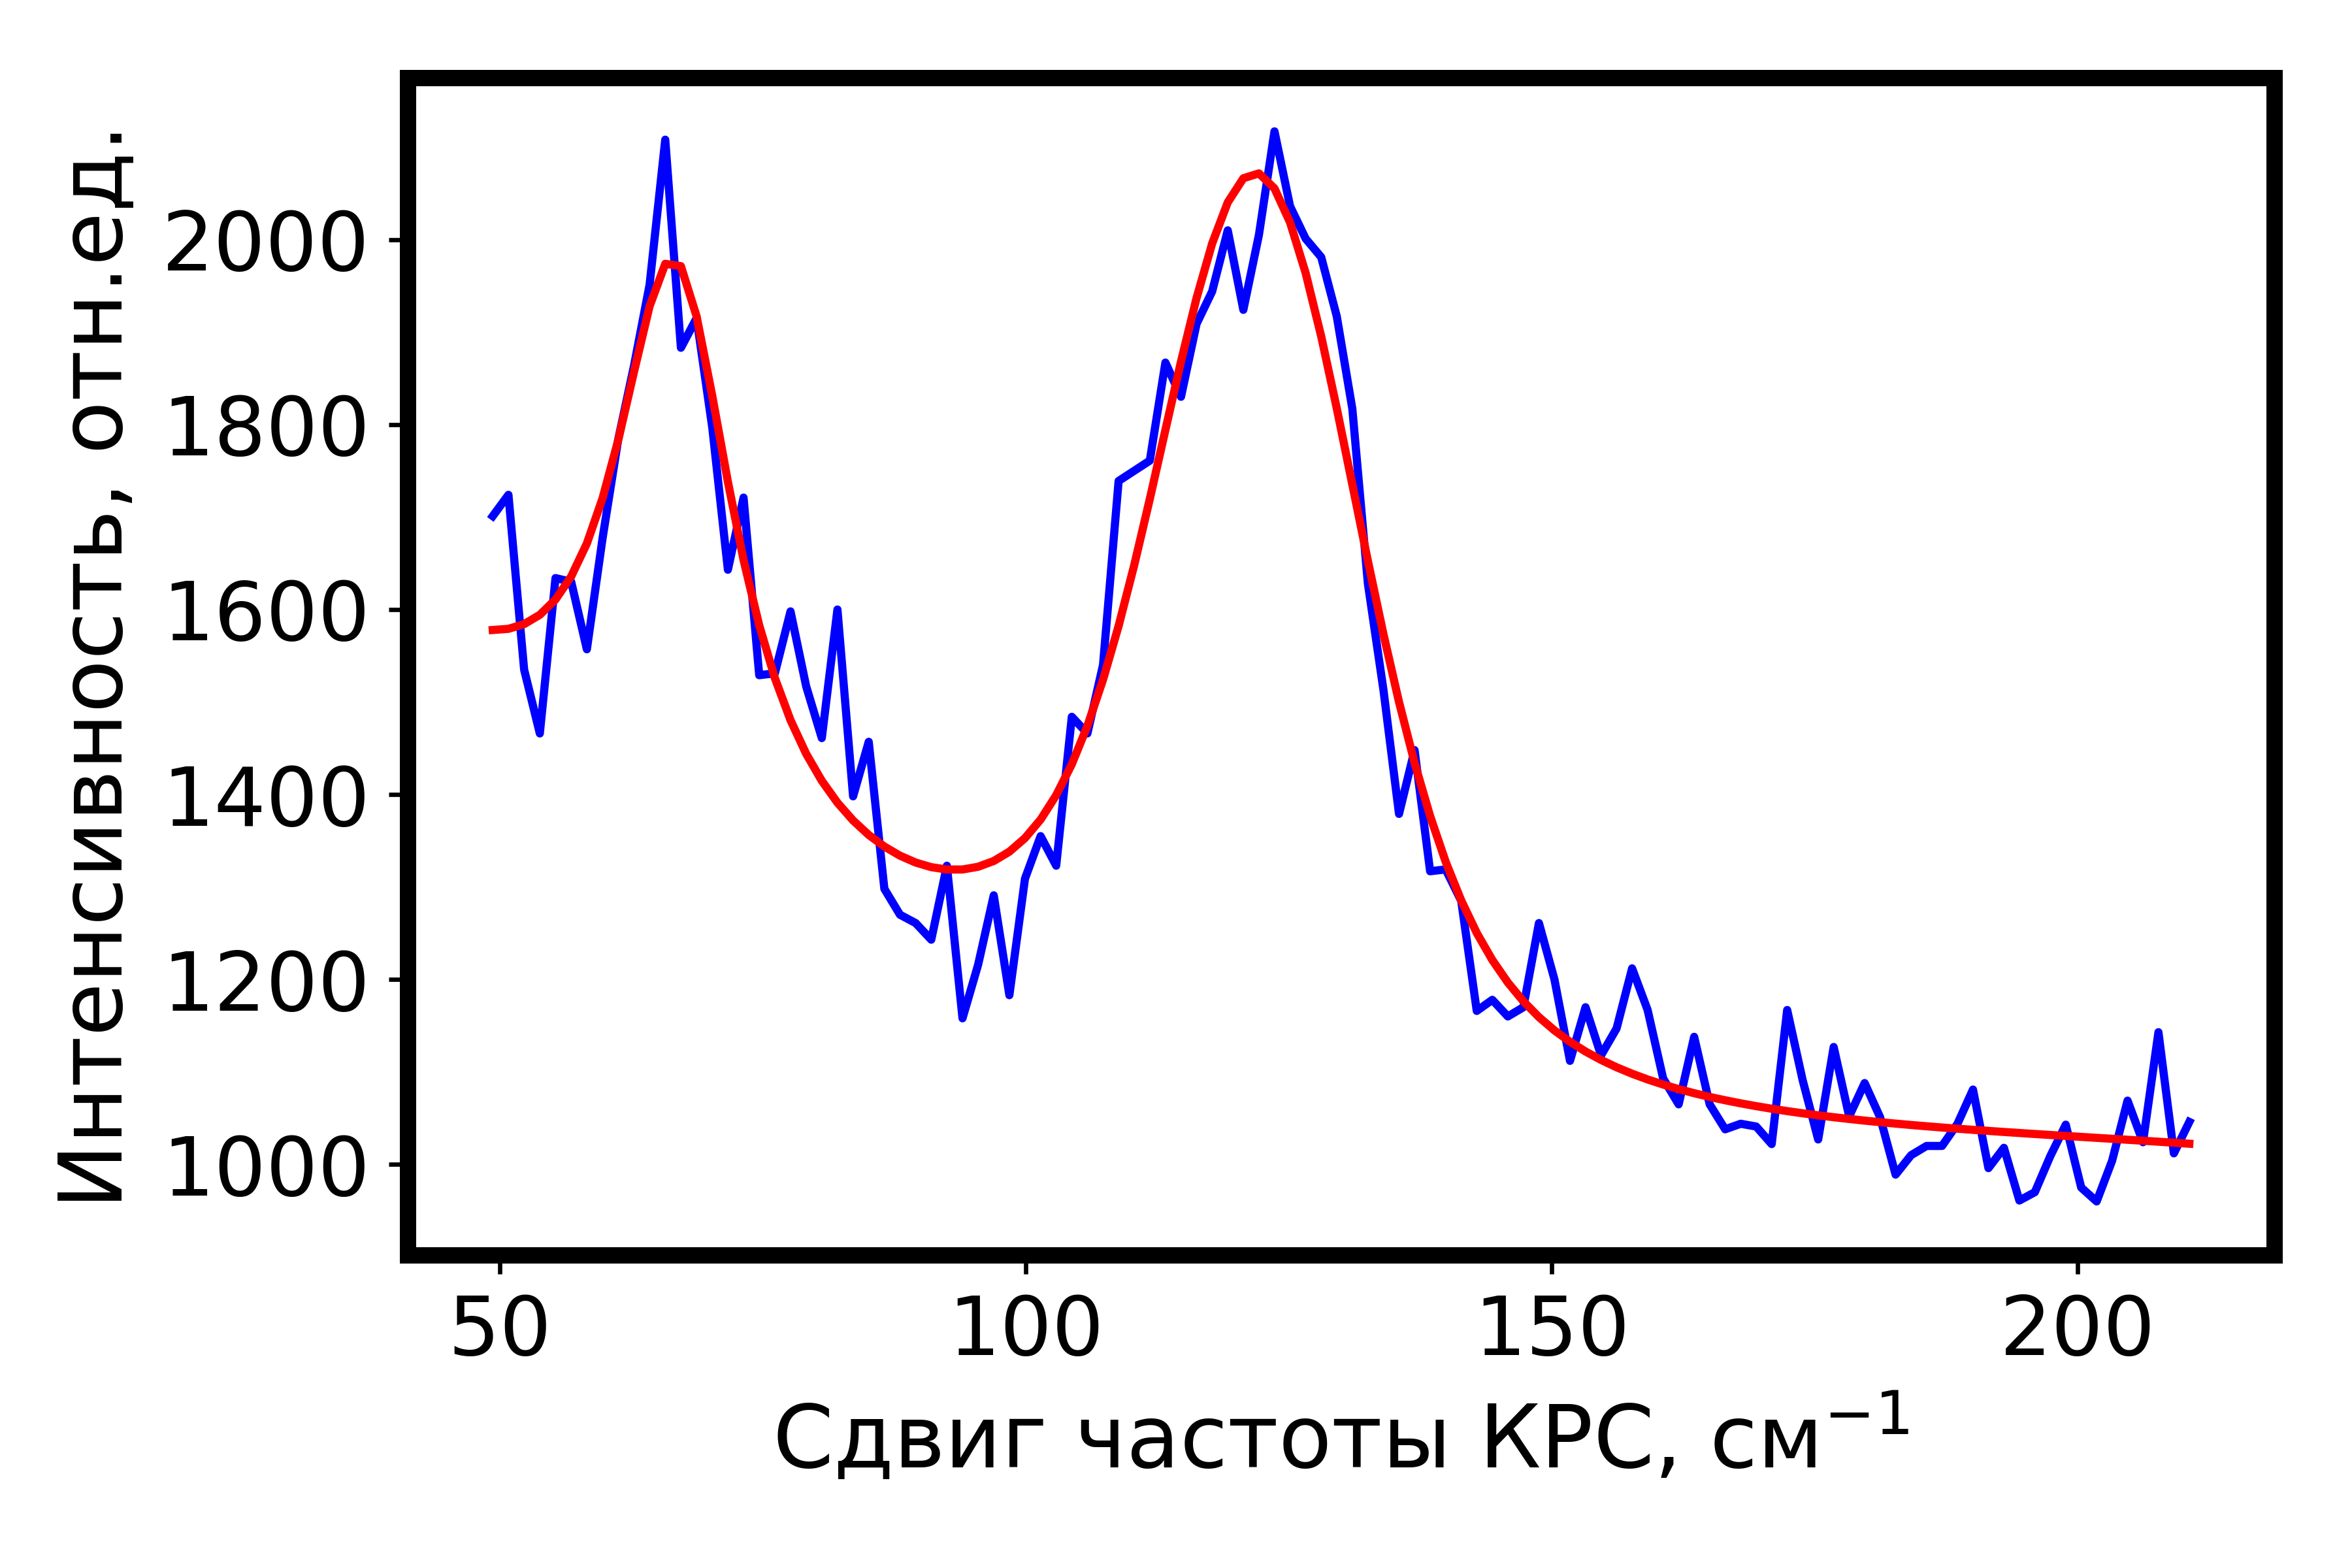
\includegraphics[width=0.9\linewidth]{raman_25_CuAsS3} \\ а)
  \end{minipage}
  \vfill
  \begin{minipage}[ht]{0.9\linewidth}\centering
    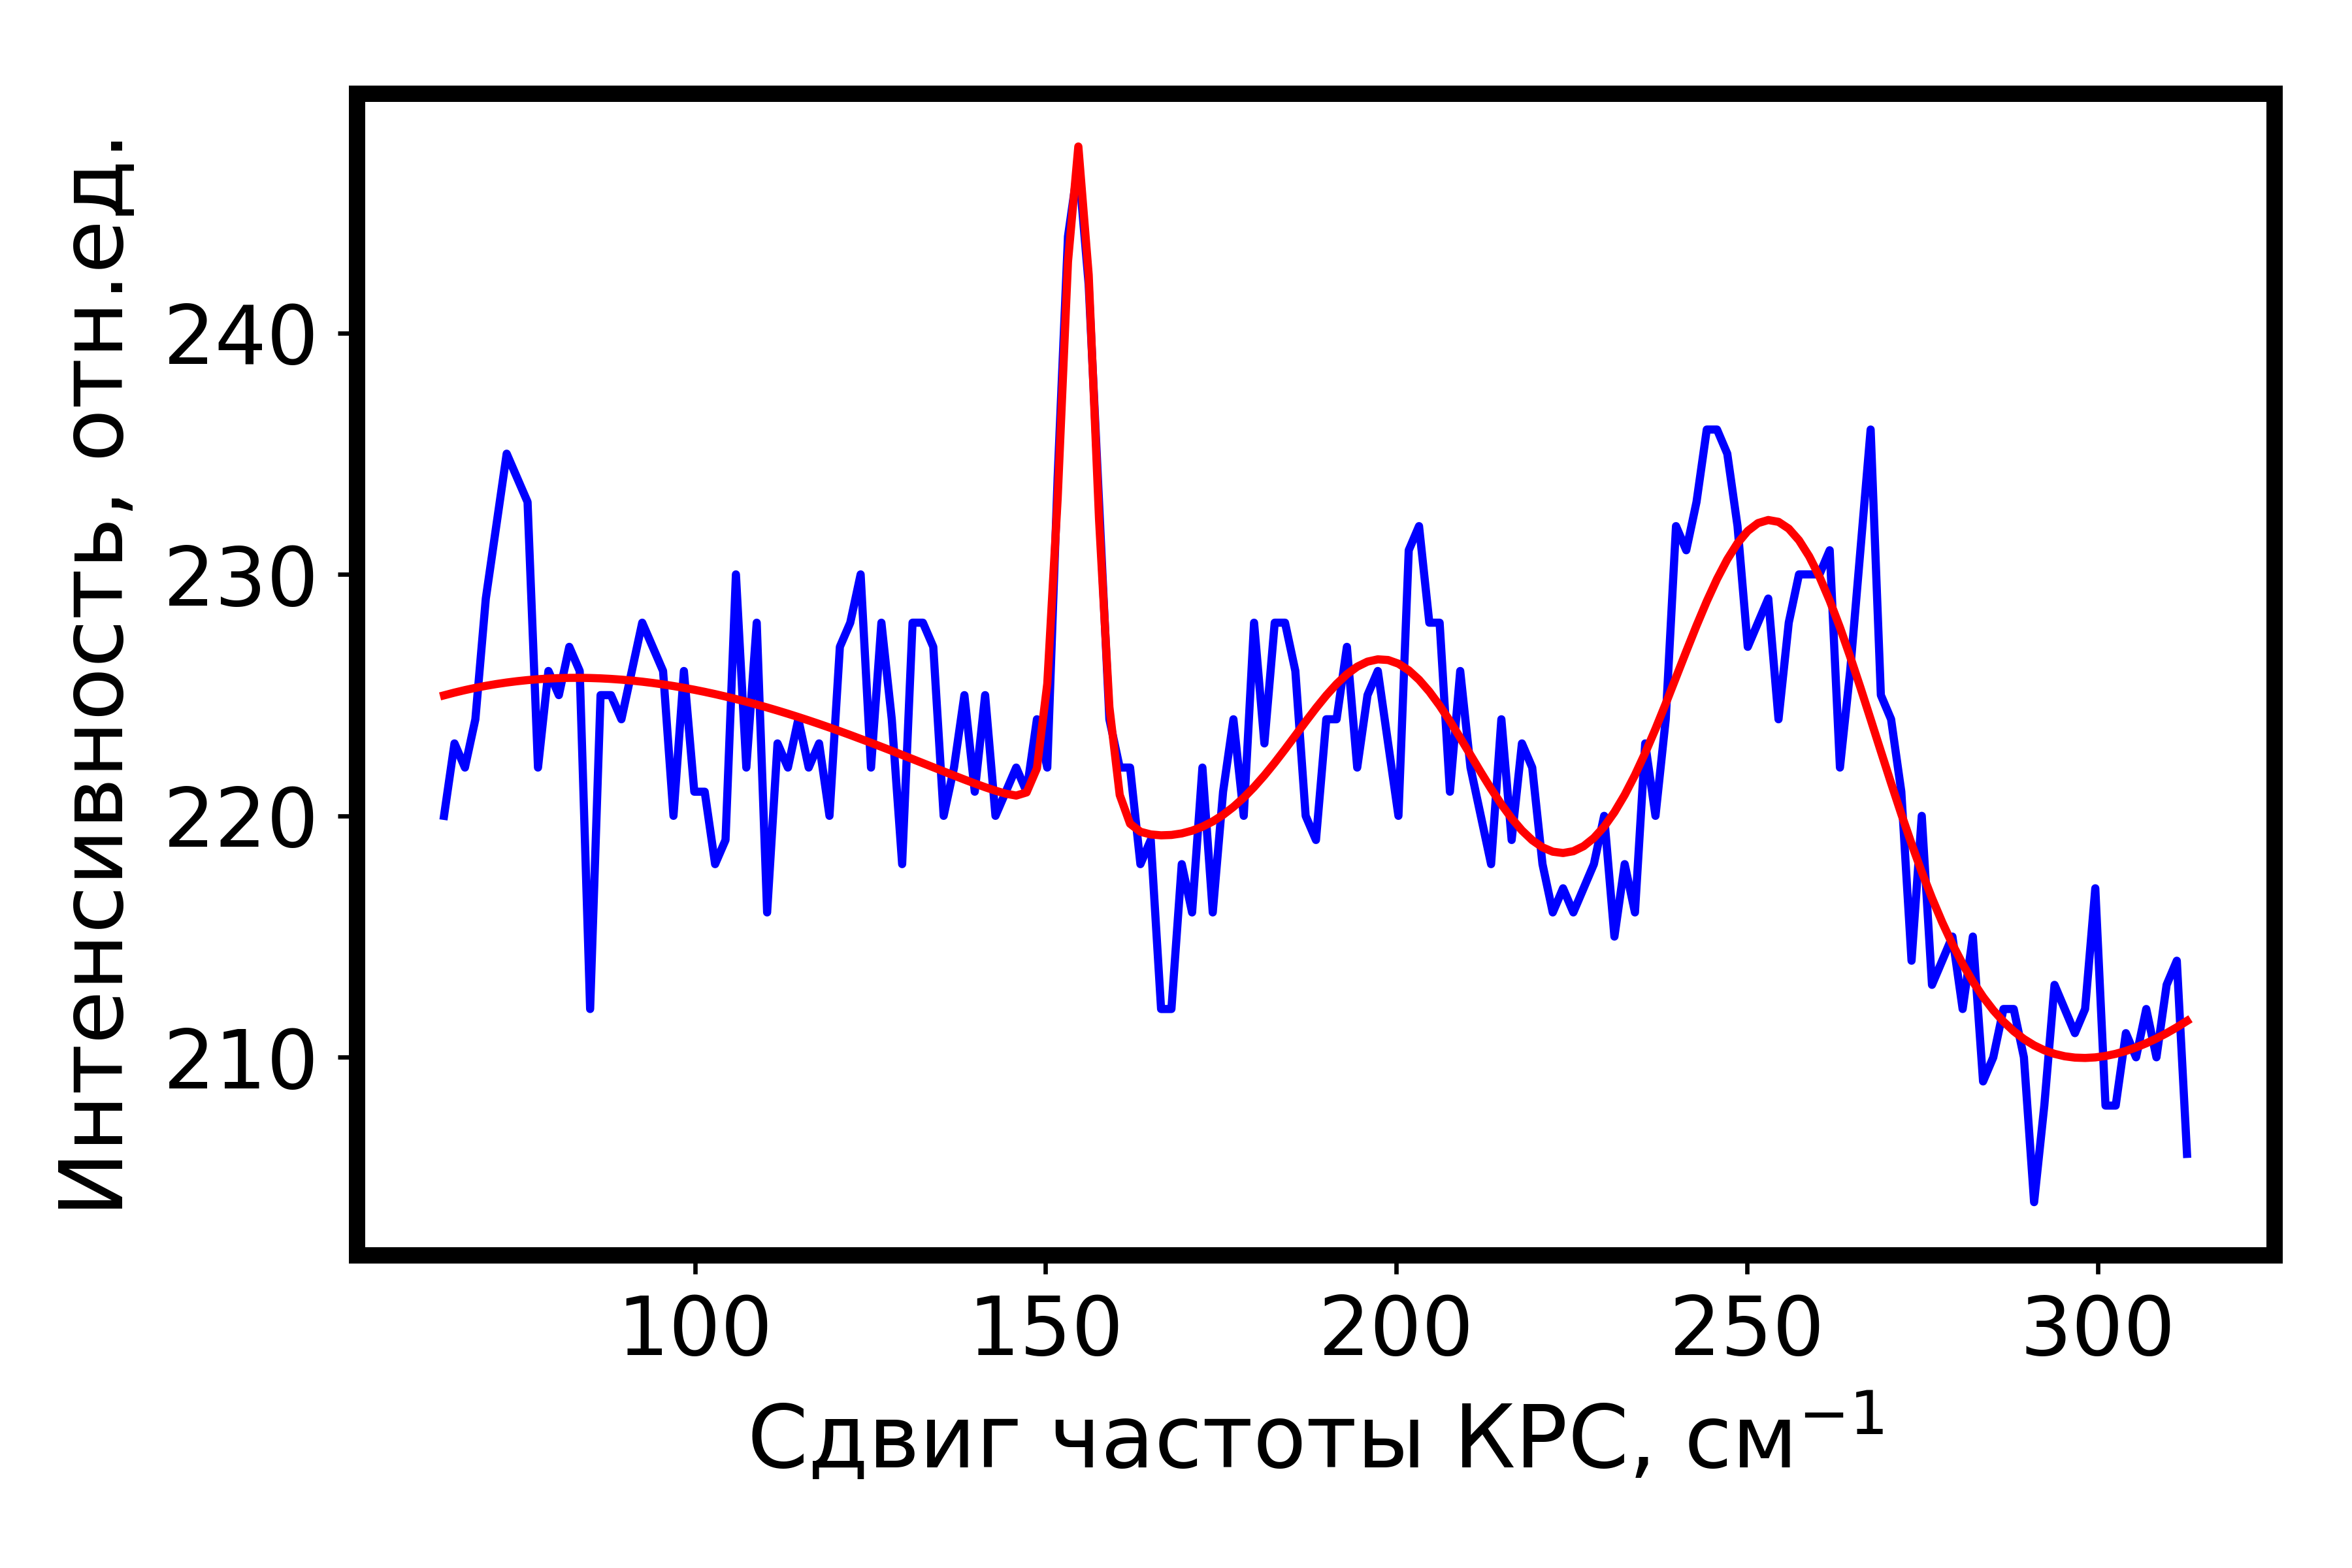
\includegraphics[width=0.9\linewidth]{raman_288_Cu3AsSe3} \\ б)
  \end{minipage}

      \caption[Графики спектров комбинационного рассеяния соединений Cu\textsubscript{12}As\textsubscript{4}S\textsubscript{13} (а) и  Cu\textsubscript{3}AsSe\textsubscript{3} (б)]{Графики спектров комбинационного рассеяния соединений Cu\textsubscript{12}As\textsubscript{4}S\textsubscript{13} (а) и  Cu\textsubscript{3}AsSe\textsubscript{3} (б)}
    \label{img:raman1}
\end{figure}

\begin{figure}[p!]
  \begin{minipage}[ht]{0.9\linewidth}\centering
    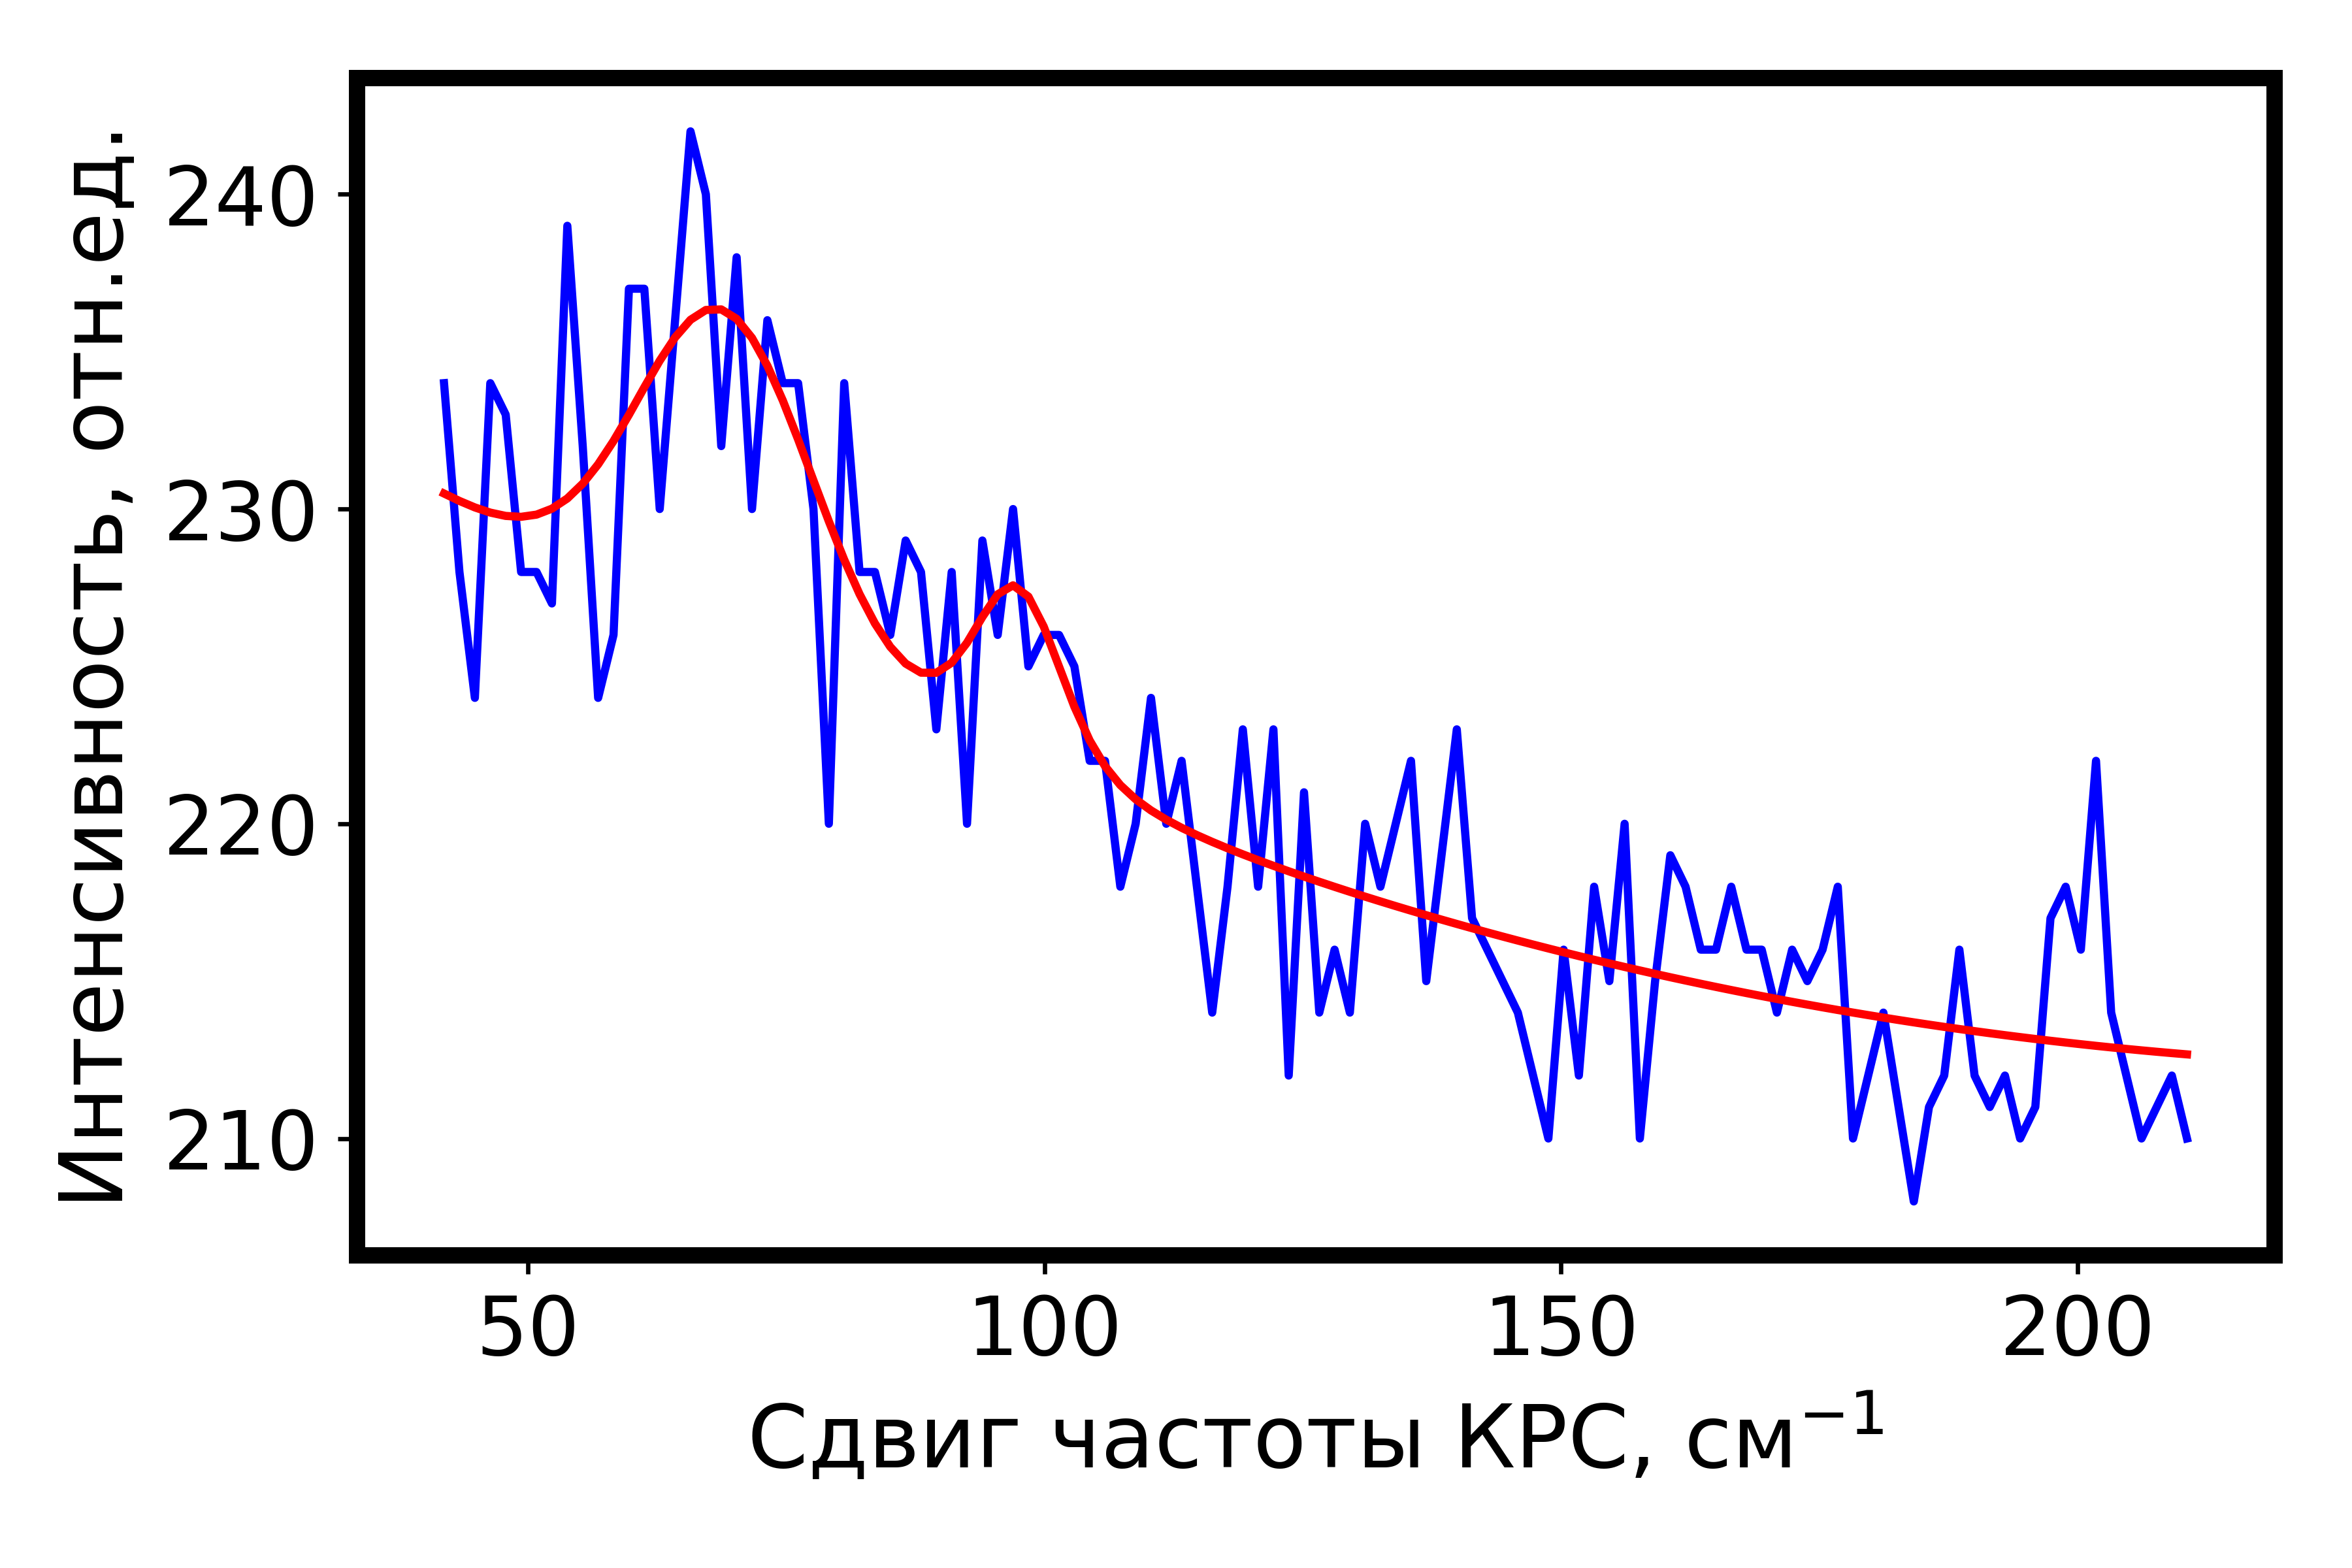
\includegraphics[width=0.9\linewidth]{raman_206_Cu3SbS3} \\ а)
  \end{minipage}
  \vfill
  \begin{minipage}[ht]{0.9\linewidth}\centering
    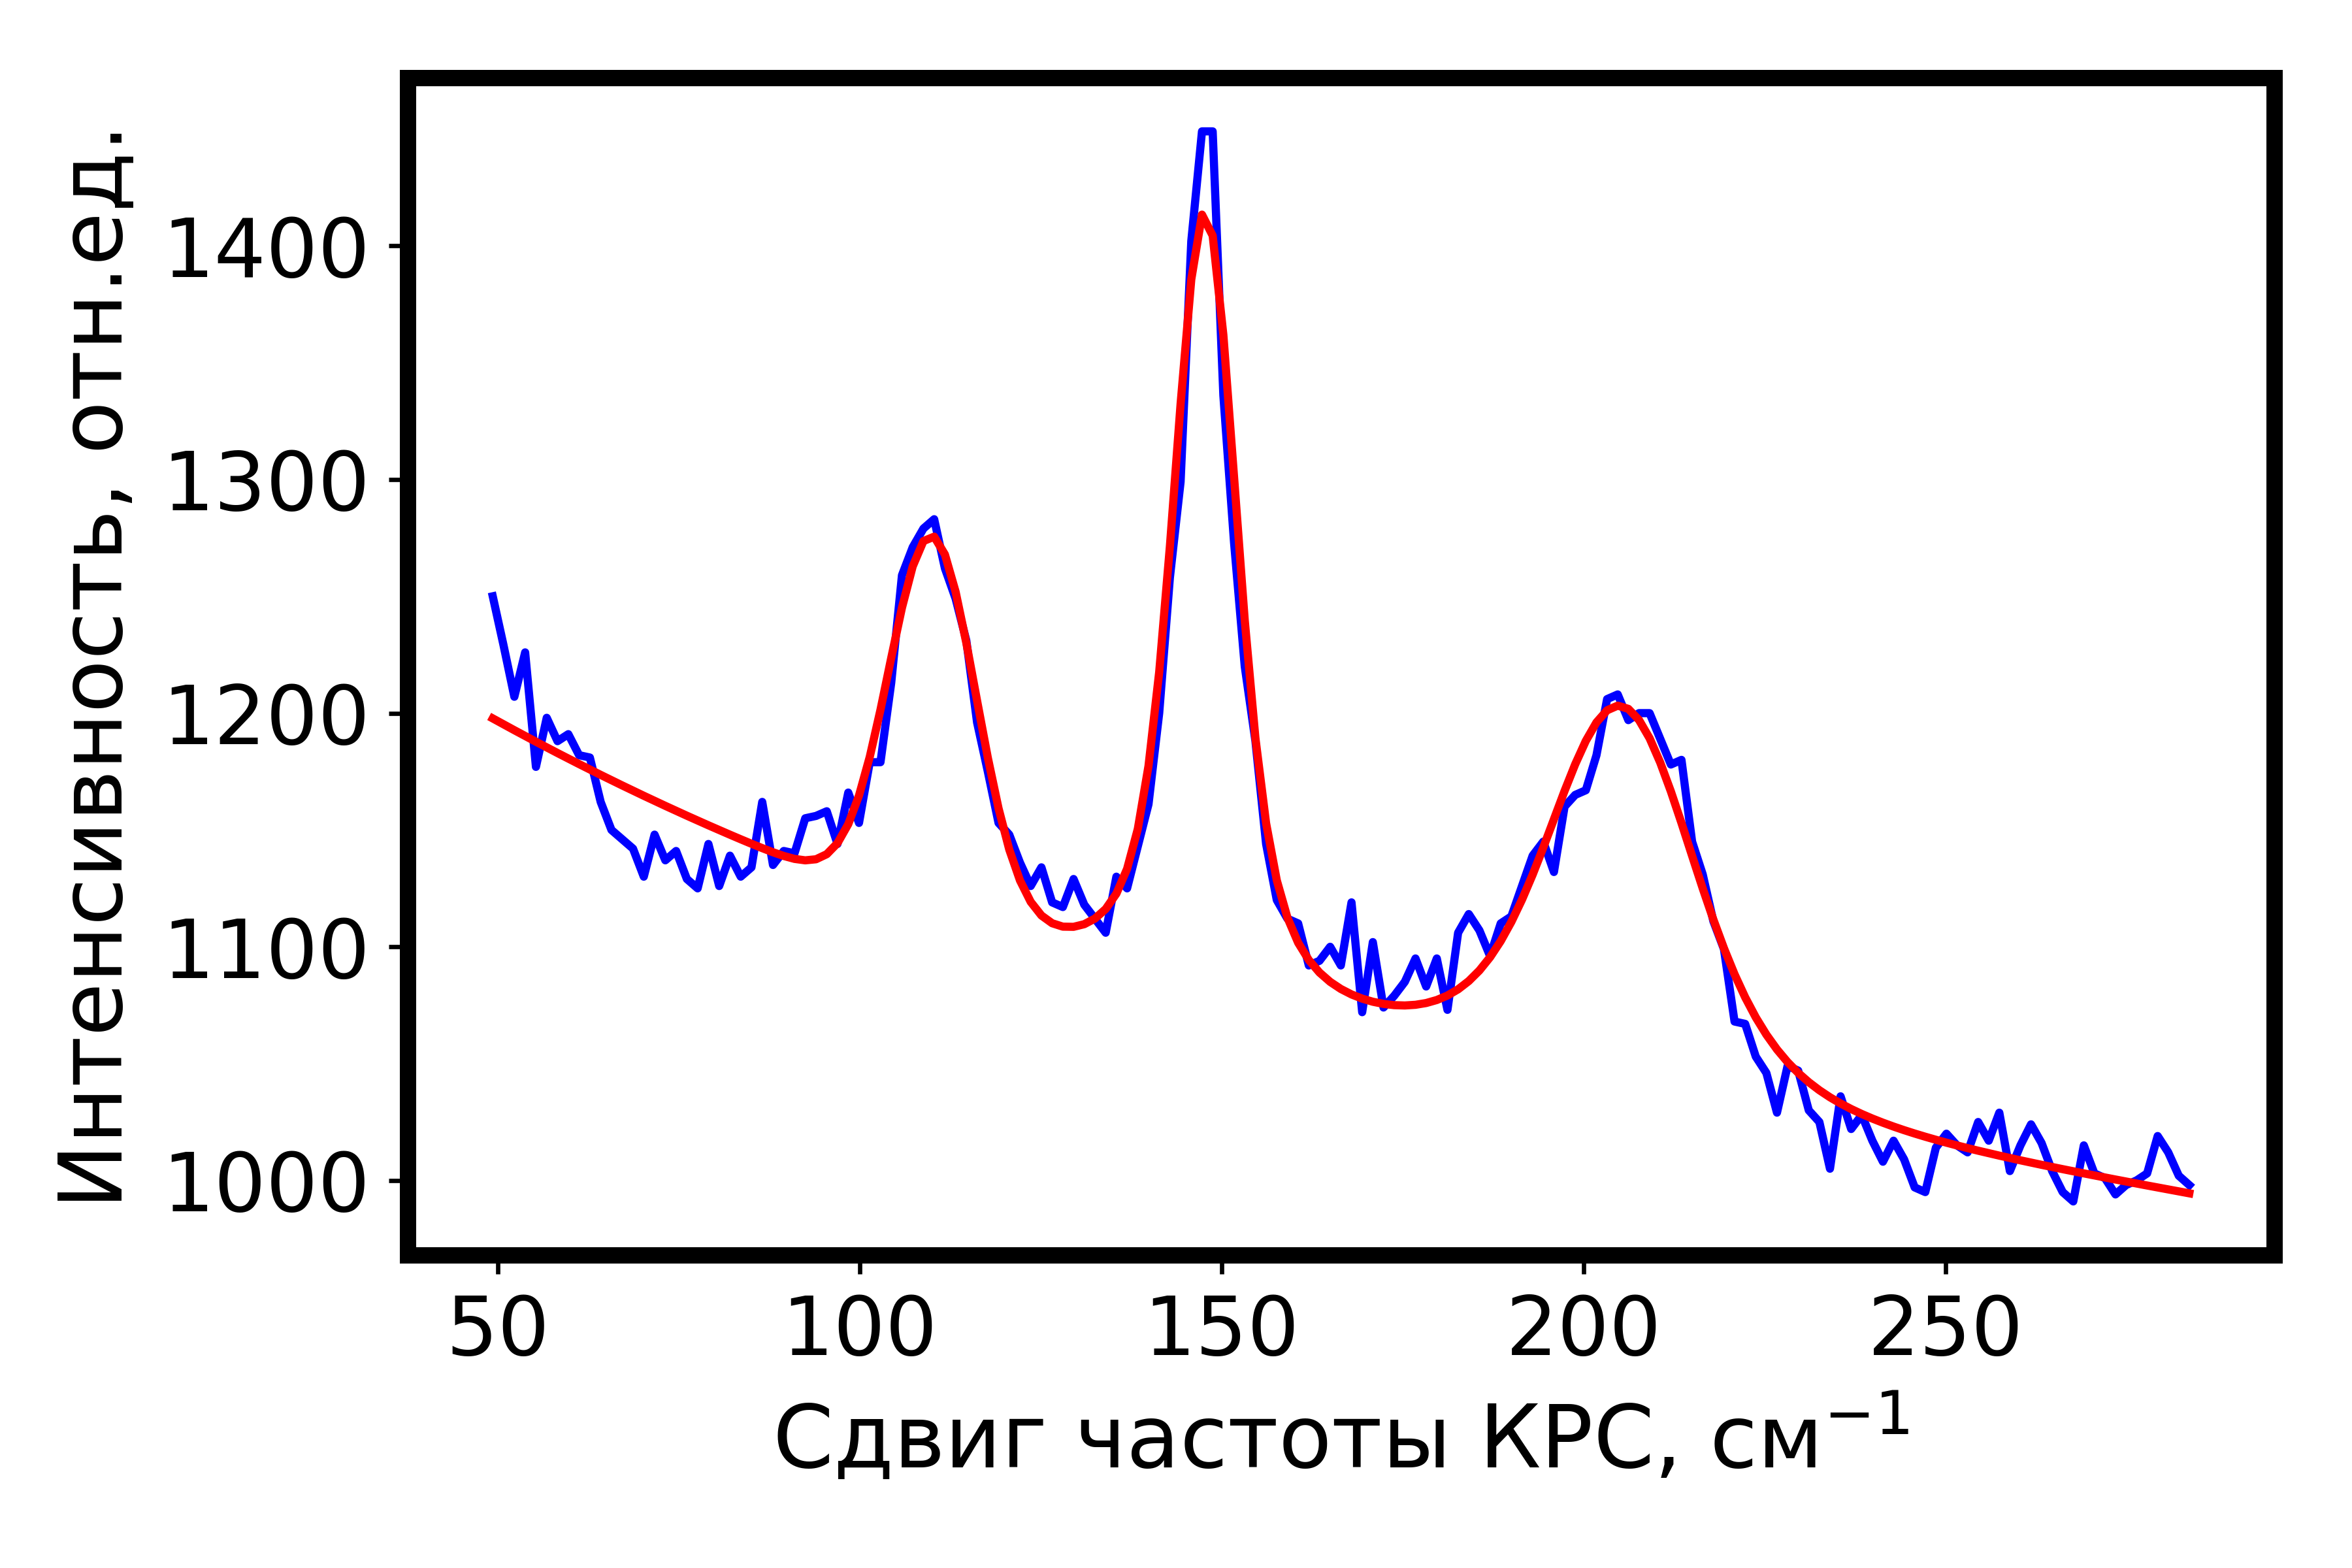
\includegraphics[width=0.9\linewidth]{raman_209_Cu3SbSe3} \\ б)
  \end{minipage}

      \caption[Графики спектров комбинационного рассеяния соединений Cu\textsubscript{12}Sb\textsubscript{4}S\textsubscript{13} (а) и Cu\textsubscript{3}SbSe\textsubscript{3} (б)]{Графики спектров комбинационного рассеяния соединений Cu\textsubscript{12}Sb\textsubscript{4}S\textsubscript{13} (а) и Cu\textsubscript{3}SbSe\textsubscript{3} (б)}
    \label{img:raman2}
\end{figure}


\newpage

\section{Температурные зависимости теплоёмкости Cu\textsubscript{12}As\textsubscript{4}S\textsubscript{13} и Cu\textsubscript{3}AsSe\textsubscript{3}} \label{sect4_4}

На рис. \ref{img:heat} представлена экспериментальная и теоретическая зависимость теплоёмкости  образца от температуры, полученная методом релаксации теплового импульса для образцов Сu\textsubscript{12}As\textsubscript{4}S\textsubscript{13} и Cu\textsubscript{3}AsSe\textsubscript{3}.
На рисунке \ref{img:heat}(а) показана экспериментальная зависимость теплоёмкости от температуры для синтетического теннантита Сu\textsubscript{12}As\textsubscript{4}S\textsubscript{13}. На графике функции наблюдаются отклонения от нормального хода теплоёмкости в диапазоне от 150 до 190 и при 285~К. Синим цветом обозначена расчётная функция теплоёмкости от температуры с тремя дополнительными осцилляторами Эйнштейна. Температура Дебая для Cu\textsubscript{12}As\textsubscript{4}S\textsubscript{13} составляет 623~К, характерные температуры эйнштейновских осцилляторов, которые составляют 65, 124 и 220~К. Температура 65~К соответствует энергии активации спин-решеточной флуктуации\cite{Gainov2008,Gainov_2006}, 124~К "--- характерному максимуму на графике зависимости магнитной восприимчивости и изменению параметра атомного смещения для позиции S(2), 220~К "--- особенностям температурной зависимости коэффициента упругой податливости\cite{bab_81}.

На рисунке \ref{img:heat}(б) представлена экспериментальная зависимость теплоёмкости от температуры для синтетического теннантита Сu\textsubscript{12}As\textsubscript{4}S\textsubscript{13}. На графике функции наблюдаются отклонения от нормального хода теплоёмкости в диапазоне от 150 до 190 и при 285 К. Синим цветом обозначена расчётная функция теплоёмкости от температуры с тремя дополнительными осцилляторами Эйнштейна. Температура Дебая для Cu\textsubscript{3}AsSe\textsubscript{3} составляет 500~К, характерные температуры эйнштейновских осцилляторов, которые составляют 42, 186 и 288~К.   Температуры 186 и 288~К соответствуют характерным максимумам на графике зависимости магнитной восприимчивости и  особенностям температурной зависимости коэффициента упругой податливости \cite{bab_81}.

\begin{figure}[p!]
  \begin{minipage}[ht]{0.9\linewidth}\centering
    \includegraphics[width=0.9\linewidth]{Heat_capacity_Cu12As4S13} \\ а)
  \end{minipage}
  \vfill
  \begin{minipage}[ht]{0.9\linewidth}\centering
    \includegraphics[width=0.9\linewidth]{Heat_capacity_Cu3AsSe3} \\ б)
  \end{minipage}

      \caption[Зависимость теплоёмкости образцов Cu\textsubscript{12}As\textsubscript{4}S\textsubscript{13} (а) и Cu\textsubscript{3}AsS\textsubscript{3} (б) от температуры. Точки~"---экспериментальные данные, сплошная линия~"---модельные значения теплоёмкости]{Зависимость теплоёмкости образцов Cu\textsubscript{12}As\textsubscript{4}S\textsubscript{13} (а) и Cu\textsubscript{3}AsS\textsubscript{3} (б) от температуры. Точки~"---экспериментальные данные, сплошная линия~"---модельные значения теплоёмкости}
    \label{img:heat}
\end{figure}



\newpage

\section{Особенности теплоёмкости для образов Cu\textsubscript{12}As\textsubscript{4}S\textsubscript{13} и Cu\textsubscript{3}AsSe\textsubscript{3} } \label{sect4_5}

Данные об аномальном поведении теплоёмкости Cu\textsubscript{12}As\textsubscript{4}S\textsubscript{13} и Cu\textsubscript{3}AsSe\textsubscript{3} согласуются с опубликованными данными \cite{bab_1982,bab_81}.
В указанных работах в этих соединениях наблюдаются аномальное изменение магнитной восприимчивости, температурной зависимости коэффициента упругой податливости и отклонение от нормального хода температурной зависимости параметра кристаллической решетки.
Стоит отметить, что авторы работ \cite{bab_1982,bab_81} подразумевали наличие однофазных соединений и связывают наблюдаемые особенности с возникновением магнитного упорядочения на парамагнитных ионах Cu\textsuperscript{2+}.
Другие работы \cite{Lara-Curzio2014,Nasonova2016} на примере синтетического тетраэдрита рассматривают особенности транспортных свойств  с точки зрения наличия низкоэнергетических фононных мод в соединении. Наличие мод подтверждается на всех исследуемых в работе соединениях, что показано на рисунках \ref{img:raman1} и \ref{img:raman2}.
Авторами работ \cite{Lara-Curzio2014,Nasonova2016} установлено, что при температуре около 90 К в соединении тетраэдрита происходит переход типа металл--полупроводник. Показано, что смещение атома серы, которое происходит вдоль поверхности октаэдра Cu\textsubscript{6}, и сдвиг атома меди, который осуществляется вдоль треугольника S\textsubscript{3}, связаны с увеличением расстояния между Cu--Sb.

\begin{figure}[p!]
  \begin{minipage}[ht]{0.9\linewidth}\centering
    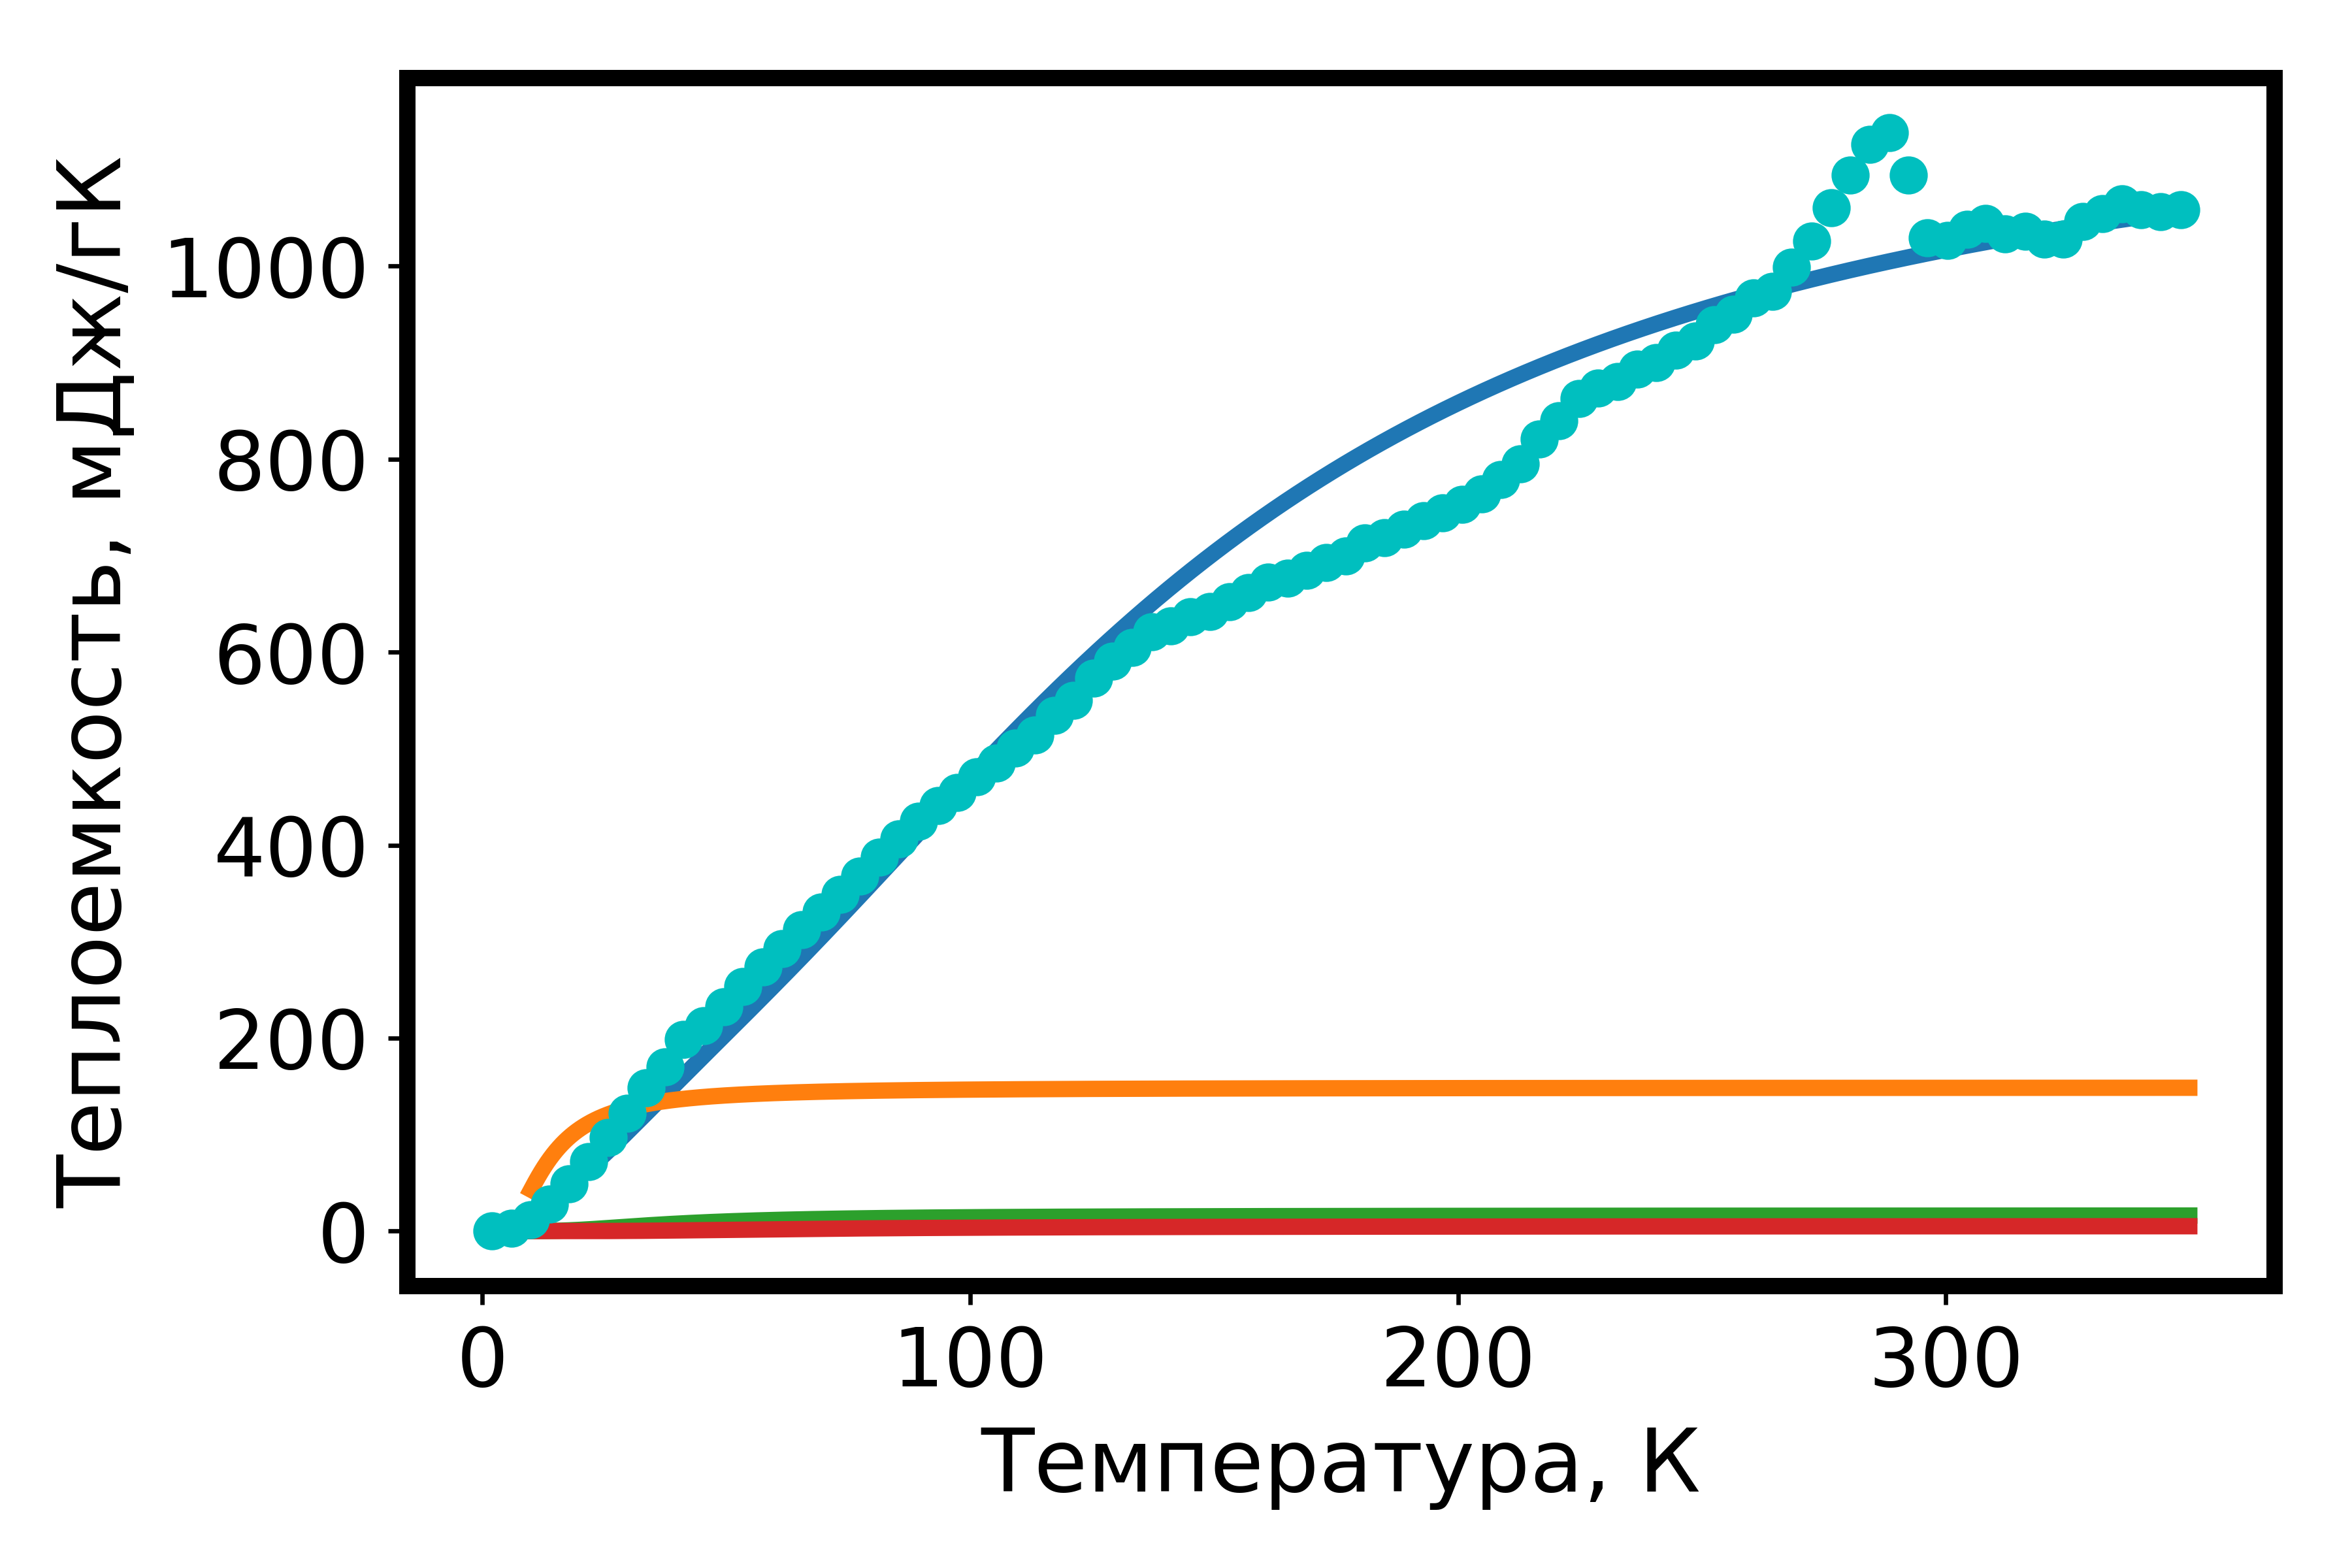
\includegraphics[width=0.9\linewidth]{Heat_capacity_cu12as4s13_with_eins} \\ а)
  \end{minipage}
  \vfill
  \begin{minipage}[ht]{0.9\linewidth}\centering
    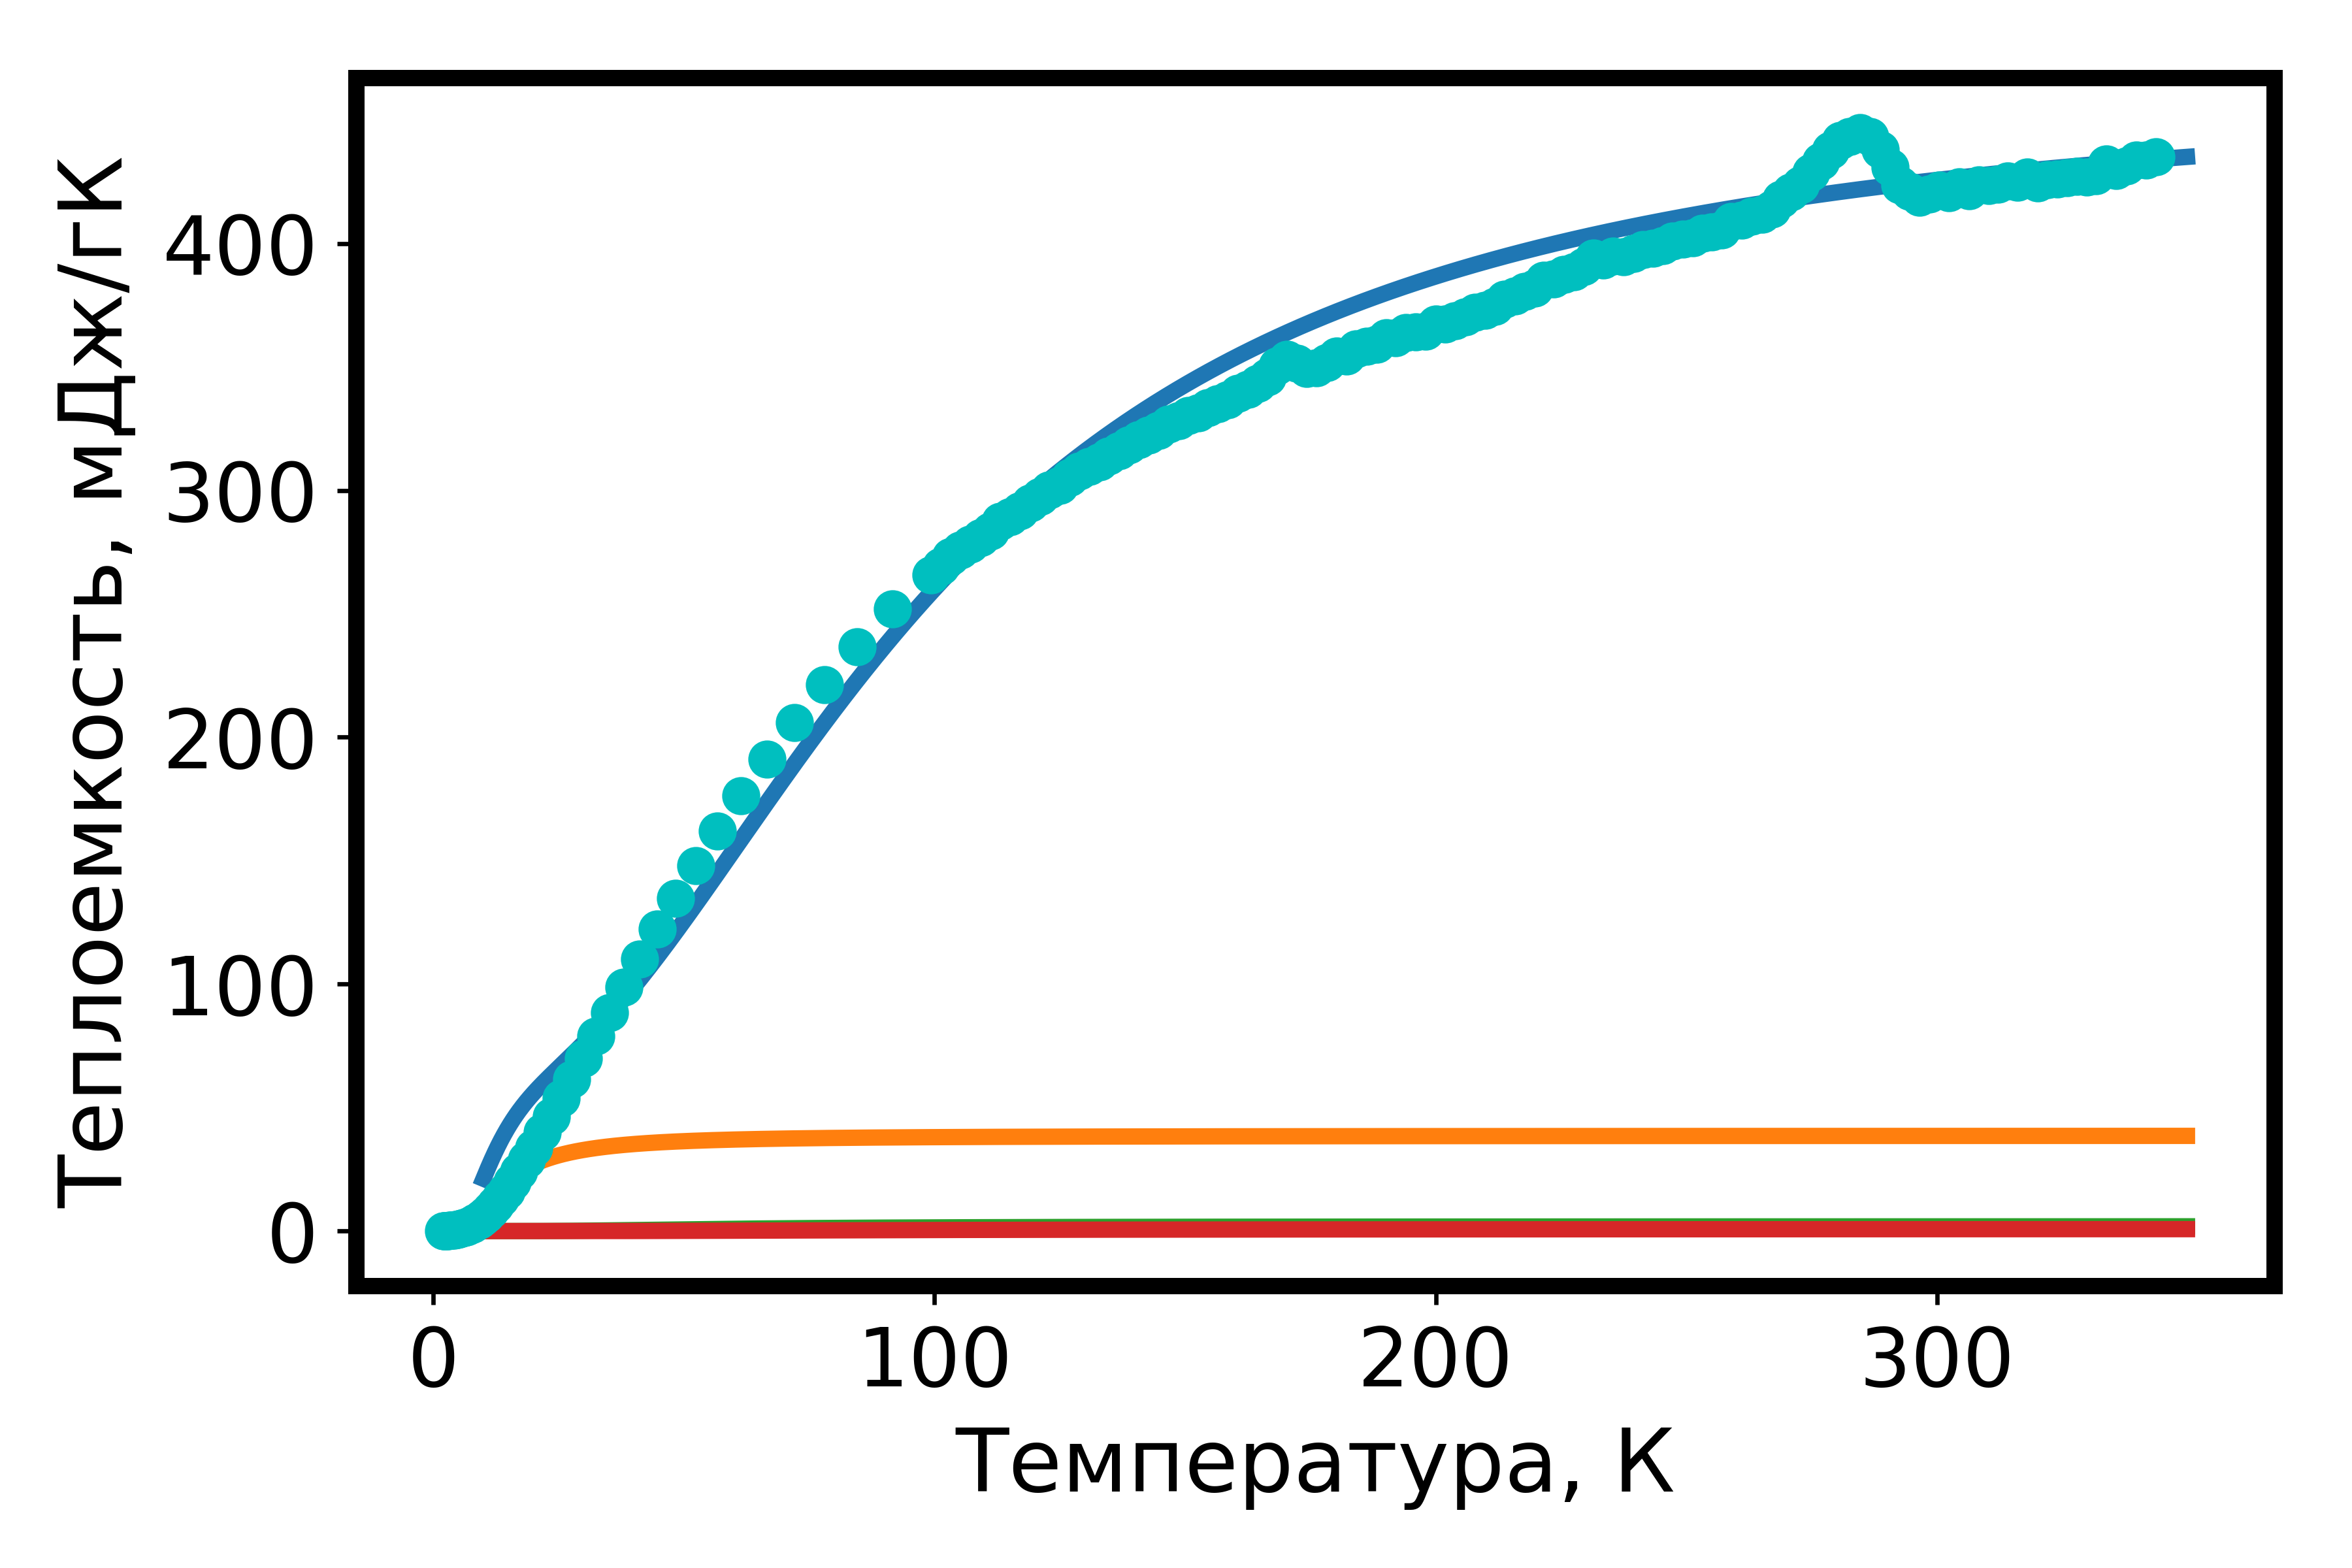
\includegraphics[width=0.9\linewidth]{Heat_capacity_cu3asse3_with_eins} \\ б)
  \end{minipage}

      \caption[Зависимость теплоёмкости образцов Cu\textsubscript{12}As\textsubscript{4}S\textsubscript{13}(а) и Cu\textsubscript{3}AsS\textsubscript{3}(б) от температуры. Точки "--- экспериментальные данные, сплошная линия "--- модельные значения теплоёмкости]{Зависимость теплоёмкости образцов Cu\textsubscript{12}As\textsubscript{4}S\textsubscript{13}(а) и Cu\textsubscript{3}AsS\textsubscript{3}(б) от температуры. Точки "--- экспериментальные данные, сплошная линия "--- модельные значения теплоёмкости}
    \label{img:heat_en}
\end{figure}


Авторы \cite{Lara-Curzio2014} отмечают, что фазовый переход в синтетическом тетраэдрите при 85~K значительно  влияет на транспортные свойства соединения: зарегистрировано резкое возрастание электрического сопротивления и максимум термоэлектрического выхода ниже фазового перехода.
Особенности физических свойств объясняются наличием статистически разориентированной позицией меди Cu(II) в структуре тетраэдрита. Стоит отметить, что в температурном структурном эксперименте для теннантита позиции меди Cu2 и Cu21, заселённость которых изменяется с измениением температуры (Рис. \ref{img:xray}б), могут быть рассмотрены как статически разоентированные позиции меди Cu(II) в тетраэдрите.
Полученные в работе температурные  зависимости теплоёмкости обладают особенностями при тех же температурах, что и в опубликованных работах.
Полученные экспериментальные зависимости описываются расчётной зависимостью теплоёмкости Дебая с дополнительными осцилляторами Эйнштейна.
Полученные подбором температуры Эйнштейна для теннантита согласуются со значениями температур Эйнштейна, полученных для атомов из структурного эксперимента.
Подобные дополнительные осцилляторы Эйнштейна, характеризующие смягчение фононных мод в кристалле\cite{bab_81}, позволяют описать полученную зависимость теплоёмкости.
По данным рентгеноструктурного анализа и квантовомеханического моделирования структура синтетического теннантита не обладает политипными модификациями. Таким образом, наблюдаемые аномалии в экспериментальных зависимостях теплоёмкостей, которые трактуются как смягчение фононных мод, представляют собой следствие суперпозиции фононных вкладов от атомов с высокими значениями коэффициентов атомарного смещения.
А наличие атомов с разными коэффициентами атомарного смещения может трактоваться, как возникновение спонтанной деформации\cite{bab_1982,bab_81}.
На рисунке \ref{img:heat_en} представлены зависимости расчётной и экспериментальной теплоёмкостей для  Cu\textsubscript{12}As\textsubscript{4}S\textsubscript{13} и Cu\textsubscript{3}AsS\textsubscript{3}.
Температура Дебая для Cu\textsubscript{12}As\textsubscript{4}S\textsubscript{13} составляет 623~К, а для Cu\textsubscript{3}AsS\textsubscript{3} "--- 500~К.
Дополнительно на каждом графике отмечены характерные температуры эйнштейновских осцилляторов, которые составляют 65, 124 и 220~К для Cu\textsubscript{12}As\textsubscript{4}S\textsubscript{13} и 42, 186 и 288~К для Cu\textsubscript{3}AsS\textsubscript{3}.
\clearpage

\newpage

\section{Закономерности изменения магнитных и некоторых физических свойств при изовалентном замещении в трёхкомпонентных халькогенидов меди} \label{sect4_4}

Все графики зависимостей магнитной восприимчивости обладают схожими особенностями при изменении температуры. Так, например, для соединения Cu\textsubscript{12}As\textsubscript{4}S\textsubscript{13} магнитное упорядочение происходит около 124~К, для Cu\textsubscript{3}AsSe\textsubscript{3} "--- около 170~К, для Cu\textsubscript{12}Sb\textsubscript{4}S\textsubscript{13}  "--- около 84~К и для Cu\textsubscript{3}SbSe\textsubscript{3}"--- около 170~К.

Согласно данным в работе \cite{Nasonova2016}, для синтетического теннантита и синтетического тетраэдрита, изменение магнитной восприимчивости вызвано изменением значения коэффициента атомного смещения для позиции S(2). Сдвиг температуры упорядочения с 124 до 84~К может быть вызван изменением локального окружения атома в позиции S(2) при изовалентном замещении As на Sb.
При подобном замещении в соединениях Cu\textsubscript{3}AsSe\textsubscript{3} и Cu\textsubscript{3}SbSe\textsubscript{3} аналогичного изменения не наблюдается. Этот факт может свидетельствовать о другом механизме фазового превращения или о многообразии возможных фазовых превращений в сложных халькогенидах меди ввиду наличия сложной ионно-ковалентной связи.

Косвенно наличие подобных связей подтверждают низкоэнергетические фононные моды обнаруженные в спектрах комбинационного рассеяния. Следует отметить, что энергия пиков для соединения Cu\textsubscript{12}Sb\textsubscript{4}S\textsubscript{13} составляет 8.5  и 12~мэВ, что находится в хорошем согласии с опубликованнымим теоретическими\cite{Lai_2015} и экспериментальными\cite{May2016} данными.

В литературе встречаются описание механизма антиферромагнитного упорядочения в сложных халькогенидах меди. Предположение о существовании антиферромагнитного упорядочения через Cu--S--Cu, вводится по аналогии с антиферромагнитным упорядочением Cu--O--Cu\cite{Crawford1976} c характерным $\phi$~=~96.94\textsuperscript{ $\circ$ }. По данным структурного исследования для синтетического теннантита в структуре возникает характерный $\phi$~=~96.01\textsuperscript{ $\circ$ } для Cu--S--Cu между позициями Cu21, S2 и Cu21. Также в литературе описывается механизм\cite{Gainov2008,Gainov_2006} перепрыгивания спина электрона между CuS\textsubscript{3} через S\textsubscript{2}, который допускает возможность возникновения магнитного упорядочения. По результатам экспериментов, проведенных в рамках диссертационной работы, не удаётся подтвердить или опровергнуть это предположение. По полученным данным структурного исследования синтетического теннантита можно заключить о неоднородности электронной плотности в структуре и, как следствие, наличии парамагнетизма.


Указанное совпадение говорит о том, что в кристаллической структуре образца существуют парамагнитные ионы, которыми, как показали квантовомехачиеские расчёты, могут быть атомы меди в позиции Cu(II).

\begin{table} [htbp]%
    \centering
	\caption{Значение температуры плавления, плотности и микротвёрдости для сложных соединений халькогенидов меди}%
	\label{hard}% label всегда желательно идти после caption
    \renewcommand{\arraystretch}{1.5}
	\begin{tabular}{@{}@{\extracolsep{20pt}}lllll@{}}
        \toprule     %%% верхняя линейка
    	 & Cu\textsubscript{12}As\textsubscript{4}S\textsubscript{13} &Cu\textsubscript{3}AsSe\textsubscript{3}& Cu\textsubscript{12}Sb\textsubscript{4}S\textsubscript{13} &Cu\textsubscript{3}SbSe\textsubscript{3}	\\
        \midrule
    T\textsubscript{пл}, К & 893 & 880												& 773& 753	\\ \hline
    	$ \rho$, г/см 	&  4.78$\pm$0.02	 						& 4.96$\pm$0.02												&5.82$\pm$0.02 	& 6.41$\pm$0.02 \\ \hline
    	H $\times$10\textsuperscript{7}, Н/м\textsuperscript{-2} 	& 154$\pm$18	 						& 134$\pm$10 	& 127$\pm$20			& 82$\pm$8	\\ \hline

        \bottomrule
	\end{tabular}%
\end{table}
В таблице \ref{hard} показано, как при увеличении молекулярного веса, температуры плавления и микротвёрдость исследованных соединений уменьшается, а плотность исследованных соединений возрастает. Такое поведение может свидетельствовать об уменьшении сил межатомного взаимодействия и может быть связано с металлизацией химических
связей.

Показано, что для получения соединения Cu\textsubscript{12}V\textsubscript{4}VI\textsubscript{13} предпочтительным является синтез из
исходной шихты с избытком по легколетучему компоненту, с последующей закалкой и
дополнительным отжигом в течении 120 часов при температуре 500 К.
\clearpage

\newpage
